%%%%%%%%%%%%%%%%%%%%%%%%%%%%%%%%%%%%%%%%%%%%%%%%%%%%%%%%%%%%%%%%%%%%%%%%%%%%%%%%
%2345678901234567890123456789012345678901234567890123456789012345678901234567890
%        1         2         3         4         5         6         7         8
\documentclass[letterpaper, 10 pt, conference]{ieeeconf}   % Comment this line out if you need a4paper
% \usepackage[UTF8]{ctex}
\usepackage{cite}
\usepackage{amsmath}
\usepackage{amsfonts}
\usepackage{steinmetz}
\usepackage{graphicx}
\usepackage{subfigure}
\usepackage{adjustbox}
\usepackage{multirow}
\usepackage{colortbl}
\usepackage{caption}
% \usepackage{subcaption}
\usepackage{hyperref}
% \usepackage[OT1]{fontenc} 
% \usepackage[colorlinks,
%             linkcolor=blue,
%             anchorcolor=blue,
%             citecolor=blue]{hyperref}
%\documentclass[a4paper, 10pt, conference]{ieeeconf}      % Use this line for a4 paper
\newcommand\kevin[1]{\textcolor{black}{#1}}

\IEEEoverridecommandlockouts                              % This command is only needed if 
                                                          % you want to use the \thanks command

\overrideIEEEmargins                                      % Needed to meet printer requirements.

%In case you encounter the following error:
%Error 1010 The PDF file may be corrupt (unable to open PDF file) OR
%Error 1000 An error occurred while parsing a contents stream. Unable to analyze the PDF file.
%This is a known problem with pdfLaTeX conversion filter. The file cannot be opened with acrobat reader
%Please use one of the alternatives below to circumvent this error by uncommenting one or the other
%\pdfobjcompresslevel=0
%\pdfminorversion=4

% See the \addtolength command later in the file to balance the column lengths
% on the last page of the document

% The following packages can be found on http:\\www.ctan.org
%\usepackage{graphics} % for pdf, bitmapped graphics files
%\usepackage{epsfig} % for postscript graphics files
%\usepackage{mathptmx} % assumes new font selection scheme installed
%\usepackage{times} % assumes new font selection scheme installed
%\usepackage{amsmath} % assumes amsmath package installed
%\usepackage{amssymb}  % assumes amsmath package installed

\title{\LARGE \bf
NDT-Map-Code: A 3D global descriptor for real-time loop closure detection in lidar SLAM
}

\author{Lizhou Liao$^{1}$, Li Sun$^{2,3*}$, Xinhui Bai$^{2}$, Zhenxing You$^{2}$, Hongyuan Yuan$^{2}$, Chunyun Fu$^{1,4}$% <-this % stops a space
\thanks{This work was supported by the Chongqing Technology Innovation and Application Development Project under Grant CSTB2022TIAD-DEX0013.}% <-this % stops a space
\thanks{$^{1}$The College of Mechanical and Vehicle Engineering, Chongqing University, China. E-mail: 
        {\tt\small liaolizhou, fuchunyun@cqu.edu.cn}.}%
\thanks{$^{2}$The autonomous driving division, NIO.  E-mail: 
        {\tt\small kevin.sun, xinhui.bai, zhenxing.you, hongyuan.yuan@nio.com}.}%
\thanks{$^{3}$Department of Computer Science, The University of Sheffield, UK}
\thanks{$^{4}$The State Key Lab of Mechanical Transmissions, Chongqing University, China.}
\thanks{$^{*}$The corresponding author.}
}


\begin{document}



\maketitle
\thispagestyle{empty}
\pagestyle{empty}


%%%%%%%%%%%%%%%%%%%%%%%%%%%%%%%%%%%%%%%%%%%%%%%%%%%%%%%%%%%%%%%%%%%%%%%%%%%%%%%%
\begin{abstract}
% \kevin{Place recognition empowers the autonomous driving vehicle to localize in GPS-denied environments.
% There is a heavy reliance on dense-point cloud maps and 360 FOV lidars in existing research on point cloud based localization.
% Our approach, named NDT-Map-Code, is a novel NDT (Normal Distribution Transform) based global descriptor, delicately designed for underground parking-lot localization.
% NDT representation is leveraged to identify the representative patterns and these patterns are further encoded according to their spatial location (bearing, range and height). 
% NDT-Map-Code can be extracted directly from NDT point cloud without the need for dense point clouds, resulting in excellent scalability and low maintenance costs. 
% Instead of using a 360 FOV lidar mounted on the car roof, we first investigate the use of a mass-produced front-view lidar for localization. To mitigate the localization challenges caused by FOV limitations and occlusions in structures, we develop a lidar local mapping system and use the instantly built local map as observations during localization.
% The experimental results on eight testing underground parking-lots show that our method outperforms the state-of-the-art methods in the top-1 recall rate indicator.}

\kevin{Loop-closure detection, also known as place recognition, aiming to identify previously visited locations, is an essential component of a SLAM system. Existing research on lidar-based loop closure heavily relies on dense point cloud and 360 FOV lidars. This paper proposes an out-of-the-box NDT (Normal Distribution Transform) based global descriptor, NDT-Map-Code, designed for both on-road driving and underground valet parking scenarios. NDT-Map-Code can be directly extracted from the NDT map without the need for a dense point cloud, resulting in excellent scalability and low maintenance cost. The NDT representation is leveraged to identify representative patterns, which are further encoded according to their spatial location (bearing, range, and height). Experimental results on the NIO underground parking lot dataset and the KITTI dataset demonstrate that our method achieves significantly better performance compared to the state-of-the-art.}

\end{abstract}


%%%%%%%%%%%%%%%%%%%%%%%%%%%%%%%%%%%%%%%%%%%%%%%%%%%%%%%%%%%%%%%%%%%%%%%%%%%%%%%%
\section{INTRODUCTION}
%Long-term Place Recognition 在机器人以及自动驾驶领域有着非常重要的作用(例如:绑架问题中的全局定位)\cite{kim2021scan}。在绑架问题中,机器人或者车辆相当于是随机被放置在先验地图中的某个场景,没有建立与所在地图的位置关系,难以利用先验地图所提供的全局定位信息进行后续的决策规划和控制。通过将自身观测与先验地图进行匹配即识别重新访问的地点,能够获取机器人/车辆与当前地图的位置关系,从而得到机器人/车辆的全局定位。重新访问的地点所提供的观测信息与先验地图所提供的先验信息具有时间差,常常会带来光照、天气以及视角的变化,因此对于此问题的求解采用视觉的方法非常困难。然而,lidar based methods 能够有效的减少由于环境变化带来的影响,因此最近几年被广泛使用。

% \kevin{Place recognition is the key technique in rescuing the kidnaped vehicle \cite{kim2021scan} or detecting loop closures in large-scale mapping, when the GPS is not available. 
% As point cloud based place recognition can address long-term challenges, it has become increasingly popular in autonomous driving scenarios, such as automated valet parking. Moreover, localization methods for large-scale applications require good adaptations of using lightweight maps since the trend of mapping will be based on onboard computation and crowd-sourced data.}

% \kevin{Existing lidar based place recognition methods\cite{kim2018scan, wang2020lidar, li2021ssc, wang2020intensity} usually convert a frame of point cloud into a two-dimensional global descriptor through polar-coordinate ROI partitioning. And rotation invariance can be achieved by column-wise shifting. 
% The main-stream methods have two limitations: firstly, the existing methods require detailed point-level geometry information hence dense point cloud map and 360 FOV lidar scan is necessary for feature representation. This will boost the requirements for onboard storage and data transmission; secondly, the existing global features are designed for outdoor scenarios, and significant adaptation is required to deal with repetitive patterns, dynamic objects and occlusion in structures for underground parking-lots localization.}

% \kevin{In this paper, we aim to propose a global descriptor, NDT-Map-Code (NDT-MC), that is highly complementary with scalable NDT point clouds built through a crowd-sourced mapping way. 
% The proposed method is devised to describe the permanent landmarks such as pillars and walls in underground parking-lots in consideration of NDT cells' geometrical shape and spatial context. 
% Our intuition is to describe the place by `what' landmarks at `where'.
% To describe `what', we classify the geometric shapes by eigenvalues of NDT cells and select effective geometrical patterns. 
% To describe `where', we propose a polar-range-height coordinates based ROI partitioning.
% Instead of focusing on structures of the largest height, we divide the entire surrounding scene structure into multiple layers according to height. 
% Afterward, both types of shapes and their heights are employed to form a multi-layer global descriptor. 
% During the query for the localization procedure, a submap is built and maintained using the lidar odometry, thereby reducing the ambiguity of visibility caused by the limited FOV of the front-view lidar.}

\kevin{Loop-closure detection is the key technique for eliminating the long-term drift in large-scale mapping when the GPS is not available (e.g. automated valet parking). Moreover, SLAM methods for large-scale applications require good adaptations of using lightweight maps since the trend of mapping will be based on onboard computation and crowd-sourced data. Existing lidar-based loop closure detection methods\cite{kim2018scan, wang2020lidar, li2021ssc, wang2020intensity} usually convert a frame of point cloud into a two-dimensional global descriptor through polar-coordinate ROI partitioning, and, the rotation invariance can be achieved by column-wise shifting. The main-stream methods have two limitations: firstly, the existing methods require detailed point-level geometry information hence dense point cloud map, and 360 FOV lidar scans are necessarily used for feature representation. This will boost the requirements for onboard storage and vehicle-cloud data transmission; secondly, in contrast to on-road driving scenarios, significant adaptation is required to deal with repetitive patterns, dynamic objects, and occlusion in structures for underground parking-lots localization and mapping.}

\kevin{This paper proposes a global descriptor, NDT-Map-Code (NDT-MC), that is highly complementary with scalable NDT point clouds built through a crowd-sourced mapping way.  The proposed method is devised to discover and describe the structural landmarks in consideration of NDT cells' geometrical shape, entropy, and spatial context.  Our intuition is to describe the place by `what' landmarks at `where'. To describe `what', we classify the geometric shapes of NDT cells. The entropy of the chosen NDT cells is considered to shortlist effective geometric patterns. To describe `where', we propose a polar-range-height-coordinate-based ROI partitioning. Instead of focusing on structures of the largest height, we divide the entire surrounding scene structure into multiple layers according to height. Afterward, both NDT's shape types and their heights are employed to formulate a multi-layer global descriptor. For front-view lidars, we employ lidar odometry to construct and maintain sub-maps. This approach can improve the limited co-visibility of the front-view-only LiDARs.}

% \kevin{The main contributions of this article are as follows:
% \begin{itemize}
%    \item
%    A novel global descriptor is devised for underground parking-lot place recognition. The proposed approach is complementary with scalable NDT point clouds, with the capability of discovering effective patterns from NDT cells and representing the scene signature through multi-layer shape-and-context encoding;
%    \item
%    A framework using front-view lidar is developed for mass-produced vehicles, by simultaneously local mapping to expend the observation spatially and temporally to discriminate the localization ambiguity;
%    \item
%    Exhaustive experiments are conducted in eight testing set at four underground parking-lots, and results show that our method achieves state-of-the-art performance.
% \end{itemize}}

The main contributions of our approach are:
\begin{itemize}
   \item
    \kevin{A novel global descriptor, NDT-MC, for underground parking scenarios. This method is complementary with scalable NDT representation, with the utilization of geometric patterns in NDT and representation of scene features through multi-layer shape and context encoding;}
   \item
   \kevin{A strengthened global descriptor - NDT-MC-plus - for on-road driving scenes. With a plug-and-use NDT entropy feature, NDT-MC's capability can be elevated  
   for scenarios with more diversities. }
   \item
   \kevin{Extensive experiments conducted on NIO underground parking-lot dataset (i.e. a collection of eight sequences in four parking lots), coupled with six sequences in the KITTI dataset, underpin the superiority of our method over state-of-the-art approaches;}
   \item 
   \kevin{We made the proposed method, together with an integrated real-time full-SLAM system, publicly accessible to the community, contributing to its potential benefits, and is subject to appropriate license agreements \url{https://github.com/SlamCabbage/NDTMC}.}
\end{itemize}


\section{RELATED WORK}
%Existing work on place recognition包含基于激光雷达的方法以及基于视觉的方法。相比于视觉的方法,lidar-based方法对于光照变换的高鲁棒性收到了持续增长的关注。对于lidar-based place recognition methods大概可以分为三类:1. Point-to-point matching;2.local descriptor;3. Global descriptor。

\kevin{Existing research on loop closure includes lidar-based methods and vision-based methods. Lidar-based methods have received increasing attention due to their robustness to lightness and illumination variance. A number of lidar-based loop closure methods have been proposed in recent years.}

%Local Descriptor。为了提升Place recognition 匹配的鲁棒性,一类通过检测出点云中的关键点,并从关键点处提取出局部描述子的方法被提取。许多关键点检测的方法在文献中被提出,如3D Sift\cite{3DSIFT},LinK3D\cite{link3d},3D-SURF\cite{3dsurf},BoW3D\cite{bow3d},Imaging-lidar\cite{ImagingLidar}。BoW3D\cite{bow3d}提取出一帧点云中的LinK3D\cite{link3d}特征,并采用Bag-of-words(BoW) model进行场景匹配。Imaging-lidar\cite{ImagingLidar}将3D点云转化为intensity range image,提取出每个image中的ORB特征,采用BoW model进行场景匹配。

\kevin{A stream of global descriptors can be constructed as a global statics of 3D local descriptors.
Several keypoint detection methods have been used, such as 3D Sift\cite{3DSIFT}, Link3D\cite{link3d}, 3D-SURF\cite{3dsurf}, BoW3D\cite{bow3d}, SHOT\cite{SHOT}, and Imaging-Lidar\cite{ImagingLidar}. After that, the methods of voting\cite{vote} and Bag-of-Words\cite{bow} are used to combine these descriptors for loop closure.}

%Global descriptor。局部描述子一类的方法需要对关键点及其对应的局部描述子进行检测与提取,这会导致计算效率非常低。相比之下,全局描述子在这计算效率上有更大的优势。最近,M2DP\cite{M2DP}通过将点云投影到多个角度的平面,生成一个向量描述子。由于这个方法对其点云的Principal Component Analysis(PCA)并不能保证两个点云能够稳健的对其,因此M2DP描述子缺乏旋转不变性。\cite{kim2018scan,li2021ssc,wang2020intensity}等方法对bird-eye view的点云进行polar-coordinate ROI partitioning生成一个二维矩阵描述子,能够通过矩阵shift实现两个描述子之间的旋转不变性。\cite{kim2018scan} 的每个 bin 保留最大高度来表示整个 bin 中的点云; \cite{li2021ssc} 和 \cite{wang2020intensity} 分别包含最多语义标签和最大强度值。\cite{wang2020lidar} 根据点的俯仰角将verticle FOV分成多层(如\cite{kim2018scan}中使用的),每层的bin被赋值0或1来表示占用和未占用。 最后,对每个极坐标 ROI 分区的不同层的 bin 进行编码,以形成最终的Lidar Iris描述符。
\begin{figure}[t]
\centering  %居中
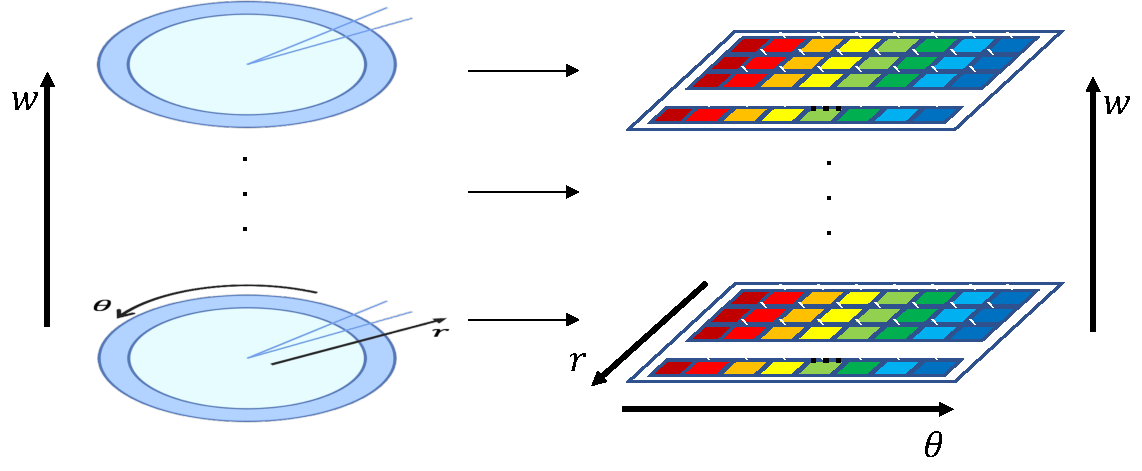
\includegraphics[width=0.98\linewidth]{TerminologyExplanation.pdf} 
 %scale为图片大小的缩放比例 res3为图片名
 %设置图像的描述(会自动生成编号)
\caption{\kevin{Polar-range-height coordinates based ROI partitioning. We first divide the 3D space according to ring, sector, and height, and the corresponding polar-range-height coordinate axes, i.e. $r$, $\theta$, and $w$, can be obtained. Afterward, the ring-sector corresponding to different heights ($w$) is transformed into a $Cartesian$ coordinate system with $\theta$ as the abscissa and $r$ as the ordinate.}}
\label{TE}
\vspace{-0.2in} 
\end{figure}
\kevin{Compared with local descriptor methods, global-based descriptors have better reproducibility in changing scenarios \cite{locus}. More recently, M2DP\cite{M2DP} generates a vector descriptor by projecting a point cloud onto a plane at multiple angles. Since this method's Principal Component Analysis (PCA) of its point cloud does not guarantee that the two point clouds can be robustly aligned, the M2DP descriptor lacks rotation invariance. Methods \cite{kim2018scan,li2021ssc,wang2020intensity} perform polar-coordinate ROI partitioning on the bird-eye viewpoint cloud to generate a two-dimensional descriptor, which can achieve rotation invariance between two descriptors through matrix shift. In \cite{kim2018scan}, each bin of the feature matrix retains the maximum height to represent all points in the bin; \cite{li2021ssc} and \cite{wang2020intensity} include the semantic labels and maximum intensity values respectively, apart from height values. Lidar Iris\cite{wang2020lidar} divides the vertical FOV into multiple layers according to the pitch angle of the point, and each layer uses the same polar-range coordinates partition as \cite{kim2018scan}. The value of a bin is assigned 0 or 1 depending on whether it is occupied or not. Finally, binary-encoded of all bins with different layers and the same polar-range partition to get the final Lidar Iris descriptor.}

%无论是局部描述子还是全局描述子都缺乏深入的描述能力。最近,通过deep learning方法学习点云的特征\cite{locus, overlaptransformer, dewan2018learning, yin2017efficient, dube2020segmap, uy2018pointnetvlad, arandjelovic2016netvlad}被运用于place recognition任务中,在描述能力上相比于传统方法有一定的提升。然而,基于learning的方法需要大量的数据进行学习以及对不同结构场景需要不同数据进行训练,在多种场景上的泛化能力不强。

%现在前向雷达的运用越来越广泛,对于轻量化点云的要求也越来越高。现有文献中针对量产车前向激光雷达的研究很少,上述方法大多是针对室外场景360度原始点云,难以在地库场景,前向雷达以及轻量化点云者三重挑战下得到预期的效果。这也激发了我们找到一种更有效的描述子去解决这三重挑战。

\kevin{Recently, deep learning methods \cite{locus, ma2022overlaptransformer, dewan2018learning, yin2017efficient, dube2020segmap, uy2018pointnetvlad, arandjelovic2016netvlad, zhou2021ndt} have been used to learn feature descriptors, and these methods have shown significant improvements in performance compared to traditional methods. However, learning-based methods show limited generalizability for novel scenes, and high computation resources are required for deployment.}

\kevin{From the literature, existing methods have three limitations: 1) firstly, most of the above methods are devised on the basis of 360-degree lidars, and it is likely to fail with a front-view lidar; 2) secondly, existing descriptors are primarily designed for outdoor on-road driving rather than underground parking scenes; 3) Existing descriptors require dense point cloud maps for feature extraction, that does not suit light-weight maps obtained by crowd-sourced mapping.}

% \begin{table}[b]
% \centering
% \caption{Comparison of storage space size of point cloud types}
% \label{table1}
% \resizebox{0.5\textwidth}{!}{
% \begin{tabular}{l|lll}
% ~             & Raw
%   Point Cloud (MB)                & NDTmap
%   2m (MB) & NDTmap
%   1m (MB)  \\ 
% \hline
% Rongke        & 2252.8   & 9.1   & 20.8  \\
% Yinwang & 889.7    & 1.7   & 5.5   \\
% Yinzuo        & 1223.7   & 4.8   & 17.1  \\
% Lixiangguoji  & 1331.2   & 4.9   & 15.6            
% \end{tabular}}      
% \end{table}

\begin{figure*}[t]
 \centering  %居中
 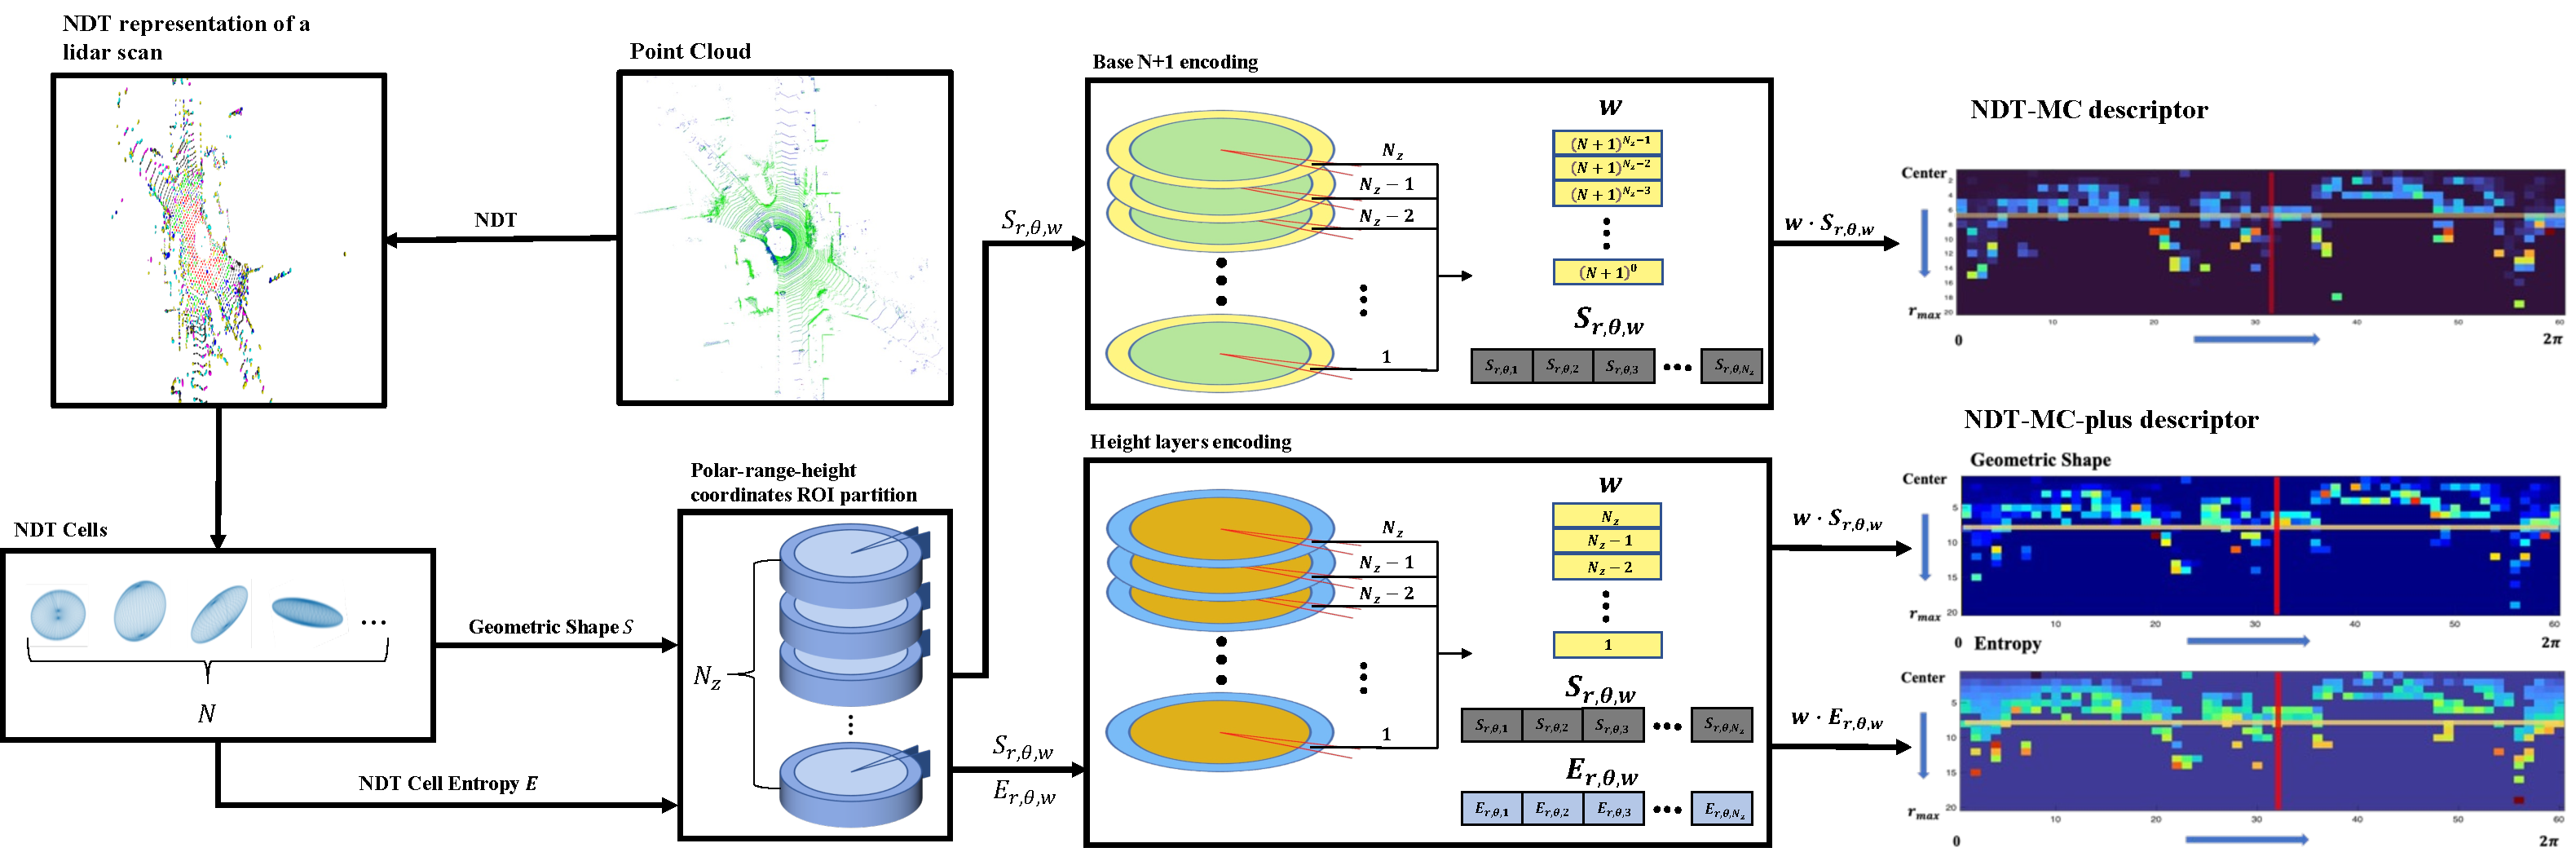
\includegraphics[width=0.98\textwidth]{pipeline.pdf} 
 %scale为图片大小的缩放比例 res3为图片名
 %设置图像的描述(会自动生成编号)
 \caption{\kevin{The overview of NDT-MC. Our approach has two variances: NDT-MC and NDT-MC-plus, which include the following steps: 1. Converting point clouds into NDT representation. 2. Calculating geometric values and entropy for each NDT cell. 3. Computing the coordinates of each NDT cell in the Polar-Range-Height coordinate system based on its mean value. Subsequently, the NDT-MC descriptor is constructed using geometric values and Base N+1 encoding, while the NDT-MC-plus descriptor is constructed using a strengthened height-layers-encoding  with entropy.}}
 \label{pipeline}
 % \vspace{-0.18in}
\end{figure*}

\section{METHODOLOGY}

\begin{figure}
 \centering
 \begin{minipage}{1\linewidth} % linewidth就是栏宽
  %\setlength{\abovecaptionskip}{-4pt}
  \subfigure[$0 < g \le 0.3$]{
   \label{g_1}
   % 图片的宽度不能设置为0.48和0.48,要留一点空间
   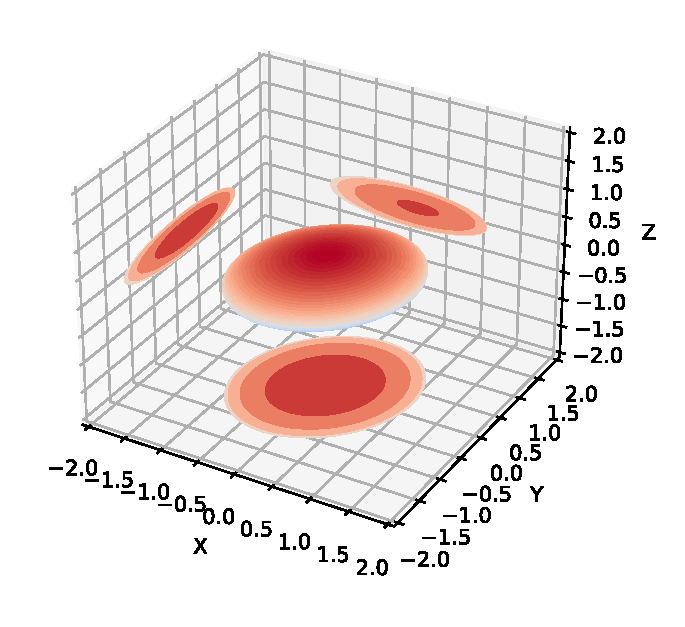
\includegraphics[width=0.49\linewidth,height=1.2in]{plane.pdf} 
  }\noindent
  \subfigure[$0.3 < g \le 0.7$]{
   \label{g_2}
   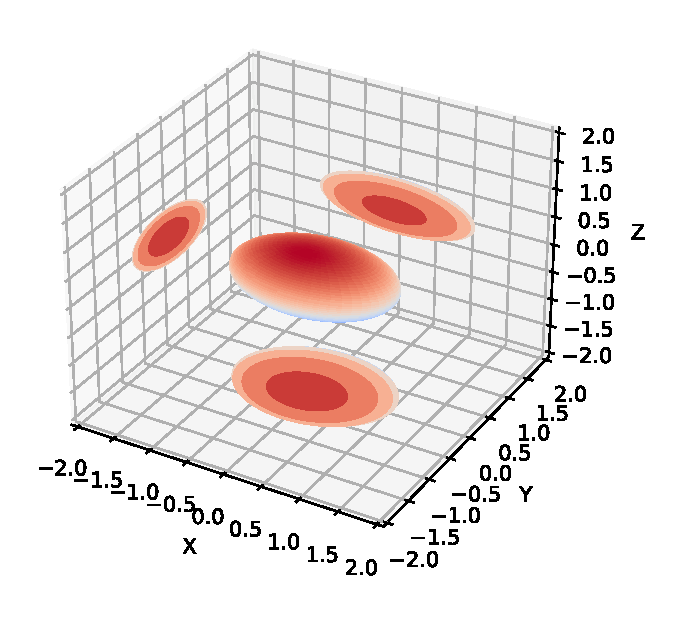
\includegraphics[width=0.49\linewidth,height=1.2in]{ellipsoid.pdf}
  }
 \end{minipage}
 \vskip -0.3cm % 用于调整两个minipage之间的垂直间距
 \begin{minipage}{1\linewidth }
  \subfigure[$0.7 < g \le 2$]{
   \label{g_3}
   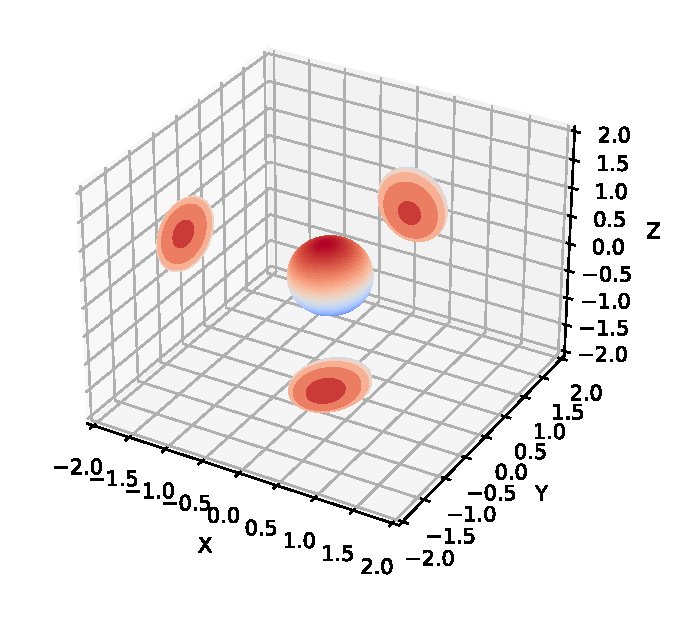
\includegraphics[width=0.49\linewidth,height=1.2in]{sphere.pdf}
  }\noindent
  \subfigure[$2 < g \le 8$]{
   \label{g_4}
   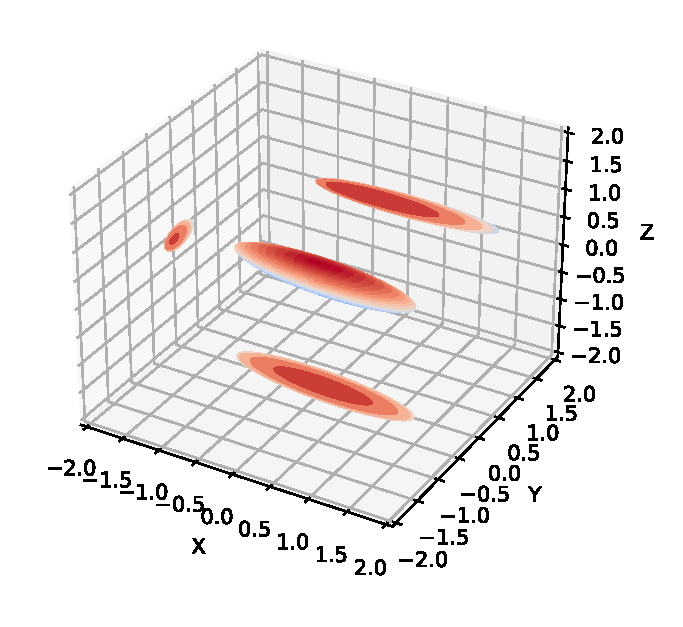
\includegraphics[width=0.49\linewidth,height=1.2in]{line.pdf}
  }
 \end{minipage}
 % \vspace{-0.18in} % 调整大标题和图片之间的距离,单位有cm in pt
 \caption{\kevin{The geometrical shape of NDT cells corresponding to different $g$ values. Four subfigures illustrate representative shapes for corresponding $g$ values, namely plane, ellipsoid, sphere, and line. In each subfigure, a 3D NDT cell is shown along with a 2D projection in the X, Y, and Z directions.}}
 % \vspace{-0.05in}  % 调整正文部分和标题(图片之间的距离)
 \label{g_figure}
\end{figure}

% \begin{figure}[t] %H为当前位置,!htb为忽略美学标准,htbp为浮动图形
% \centering %图片居中
% \includegraphics[width=1\linewidth]{./figure/Fig.1 .pdf} %插入图片,[]中设置图片大小,{}中是图片文件名
% \caption{\kevin{Place Recognition in an underground parking-lot using NDT-Map-Code (NDT-MC). The black and blue lines represent the database trajectory and the testing trajectory respectively, which are collected at different times. The red circle represents the submap of the testing data, which is built by the Lidar-inertial odometry. The green circles represent NDT submaps of the database, which can be obtained directly from a global NDT point cloud.} 
% %The red line and the green line represent the flow of testing data and database construction descriptors respectively.
% } %最终文档中希望显示的图片标题
% \label{Fig. 1} %用于文内引用的标签
%  % \vspace{-0.2in}
% \end{figure}
\begin{figure}[t] %H为当前位置,!htb为忽略美学标准,htbp为浮动图形
\centering %图片居中
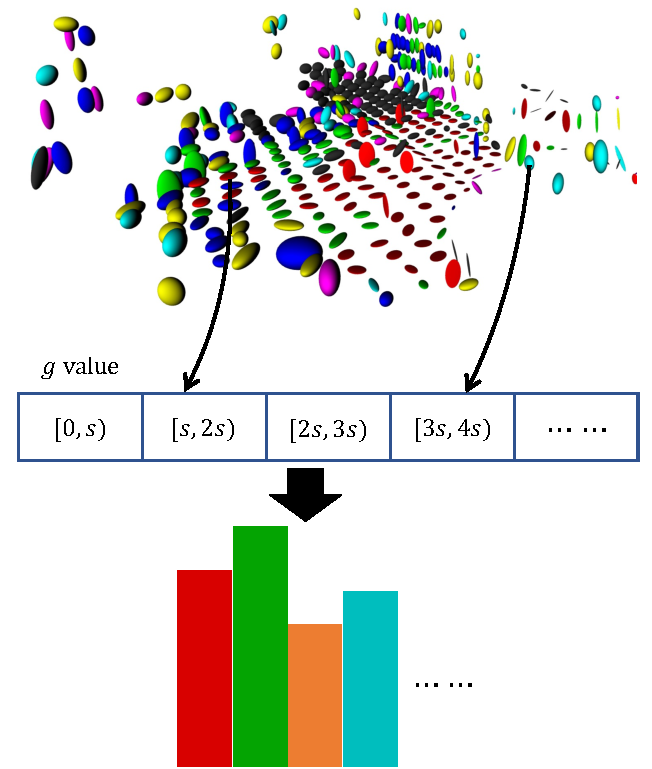
\includegraphics[height=5cm]{geometrickey.pdf} %插入图片,[]中设置图片大小,{}中是图片文件名
\caption{Construction of geometric key.} 
\label{GK} %用于文内引用的标签
 \vspace{-0.2in}
\end{figure}

\subsection{NDT represent point cloud}
\kevin{NDT is used to represent the point cloud due to its scalability in mapping large-scale scenes, as well as its advantages in noise and outlier removal and reducing the number of points to improve processing speed. To obtain an NDT point cloud, we divide the point cloud into uniformly distributed 3D grids and estimate a multivariate Gaussian for each cell. A one-pass algorithm is used to calculate the mean and covariance:}
\begin{equation}
\small
\begin{split}
\label{mean}
 (\bar{x}_i,\bar{y}_i,\bar{z}_i) = (\bar{x}_{i-1},\bar{y}_{i-1},\bar{z}_{i-1})+ \\  \frac{1}{i}(x_i-\bar{x}_{i-1},y_i-\bar{y}_{i-1},z_i-\bar{z}_{i-1}) \ \\ 
\end{split}
\end{equation}
\begin{equation}
\small
\begin{split}
\label{C_i}
C_i = C_{i-1} + \frac{i-1}{i}(x_i-\bar{x}_{i-1},y_i-\bar{y}_{i-1},z_i-\bar{z}_{i-1})^T \\ 
\cdot (x_i-\bar{x}_{i-1},y_i-\bar{y}_{i-1},z_i-\bar{z}_{i-1}) \ \\
\end{split}    
\end{equation}
\begin{equation}
\small
\begin{split}
\label{Cov_n}
{Cov}_n = \frac{C_n}{n}
\end{split}
\end{equation}
\kevin{where $\left({\bar{x}}_i,{\bar{y}}_i,{\bar{z}}_i\right)$ refers to the mean value of the previous $i$ points, and $n$ is the total number of points, $C$ is a matrix of $3\times3$, and ${Cov}_n$ represents the covariance matrix of $n$ points.}

\subsection{Polar-range-height coordinates ROI partition}

\kevin{Similar to Scan-Context-like methods, polar-range coordinates ROI partition is used to divide 3D space into rings and sectors:}
\begin{equation}
\small
\label{rlayer}
    r_k=max\left\{r_k\in\mathbb{Z}\ |\ r_k\le\frac{\sqrt{x_k^2+y_k^2}}{L_r},0\le\sqrt{x_k^2+y_k^2}\le R\right\}
\end{equation}
\begin{equation}
\small
    \Theta\left(\frac{y_k}{x_k}\right)=\left\{
    \begin{aligned}
    arctan\frac{y_k}{x_k},{0<x}_k,\ 0\le y_k \\
    arctan\frac{y_k}{x_k}+\pi,x_k < 0 \\
    arctan\frac{y_k}{x_k}+2\pi,0<x_k,y_k<0
    \end{aligned}
    \right.
\end{equation}
\begin{equation}
\small
\label{thetalayer}
    \theta_k=max\left\{\theta_k\in\mathbb{Z}\ |\ \theta_k\le\frac{\Theta\left(\frac{y_k}{x_k}\right)}{L_\theta},0\le\sqrt{x_k^2+y_k^2}\le R\right\}
\end{equation}
% 其中$L_r$和$L_\theta$分别表示极坐标的radial resolution和angular resolution,R表示允许的最大radial distance。$r_k$和$\theta_k$表示$p_k$的Polar coordinates index,其最大值分别为$N_r$和$N_\theta$. 如Fig. \ref{TE}所示,$r,\theta,w$分别为描述子构建时的三个index。
\kevin{where $L_r$ and $L_\theta$ represent the radial resolution and angular resolution of polar coordinates respectively, and $R$ represents the maximum radial distance allowed. $\theta_k$ and $r_k$ represent the polar and range coordinates indices of $p_k$, whose maximum values are $N_r$ and $N_\theta$ respectively.}
 
\kevin{Existing methods focus on describing the buildings for outdoor localization. Specifically, each bin of \cite{kim2018scan} retains the maximal height value to represent the point cloud in the entire ROI bin; \cite{li2021ssc} and \cite{wang2020intensity} include the most semantic labels and the maximum intensity value, respectively. }

\kevin{In underground parking lots, the presence of dynamic objects, such as parked cars, can significantly impact scan-context-like approaches. Moreover, due to the equivalent height of ceiling,  maximal-height-based descriptors show limited effectiveness in discriminating between different locations. }

%Similarly, in outdoor scenes, the density of scan lines from mechanical lidar decreases as the angle between the lidar and the horizontal plane increases. This results in sparser point clouds in higher areas of the frame, leading to weaker object description capabilities in those regions.

\kevin{To address these challenges, as illustrated in Fig. \ref{TE}, we propose an alternative approach to dividing the scene $p_k(x_k, y_k, z_k)$ into multiple layers based on height values with respect to the vehicle's base link. Unlike the method proposed in \cite{wang2020lidar}, we do not use pitch angles for vertical partition. Instead, we  segment the scene into layers according to the height values.}

\begin{equation}
\label{zlayer}
    w_k=max\left\{{w_k} \in \mathbb{Z} | {w_k} \leq \frac{z_k}{L_z}, 0 \leq {z_k} \leq Z \right\}
\end{equation}
\kevin{Here, $\mathbb{Z}$ means natural number, $L_z$ represents the height of each layer, $Z$ refers to the maximal $z$ value of truncated points $[0, Z]$, and $w_k$ represents the layer index to which $p_k$ belongs. }

\subsection{Classification of NDT shapes and calculation of entropy}
\begin{figure*}[t]
    \centering
    \subfigure[Rongke]{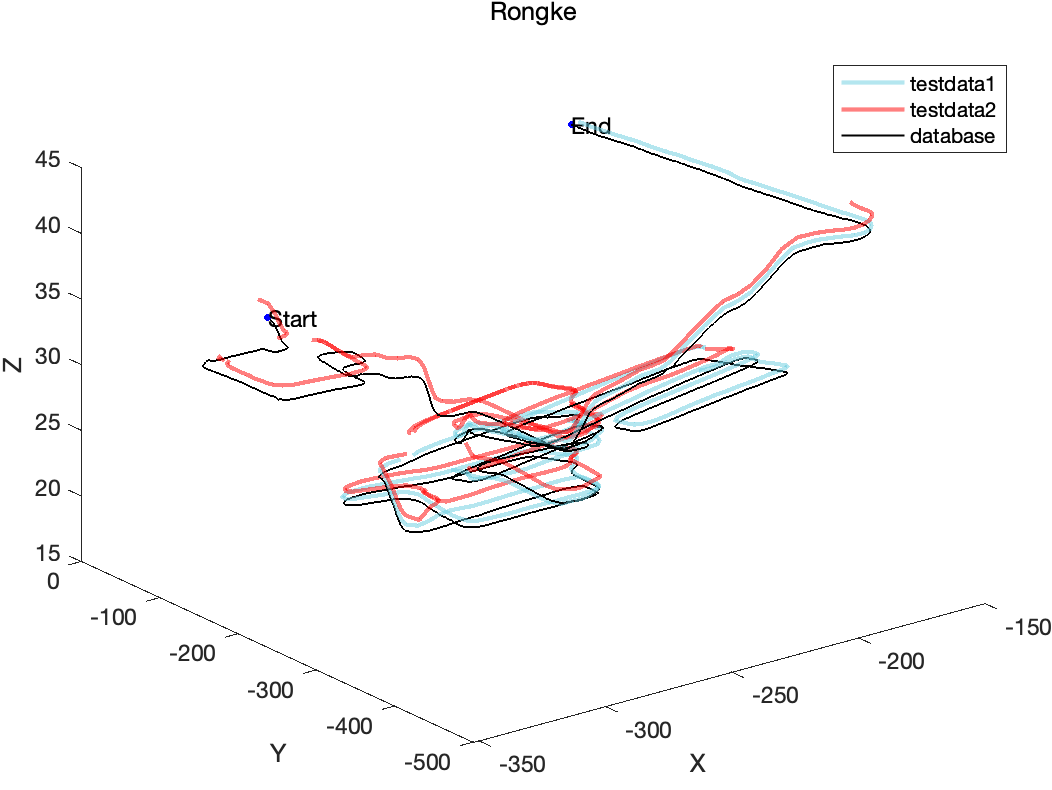
\includegraphics[width=0.24\textwidth]{Rongke.pdf}} 
    \subfigure[Lixiangguoji]{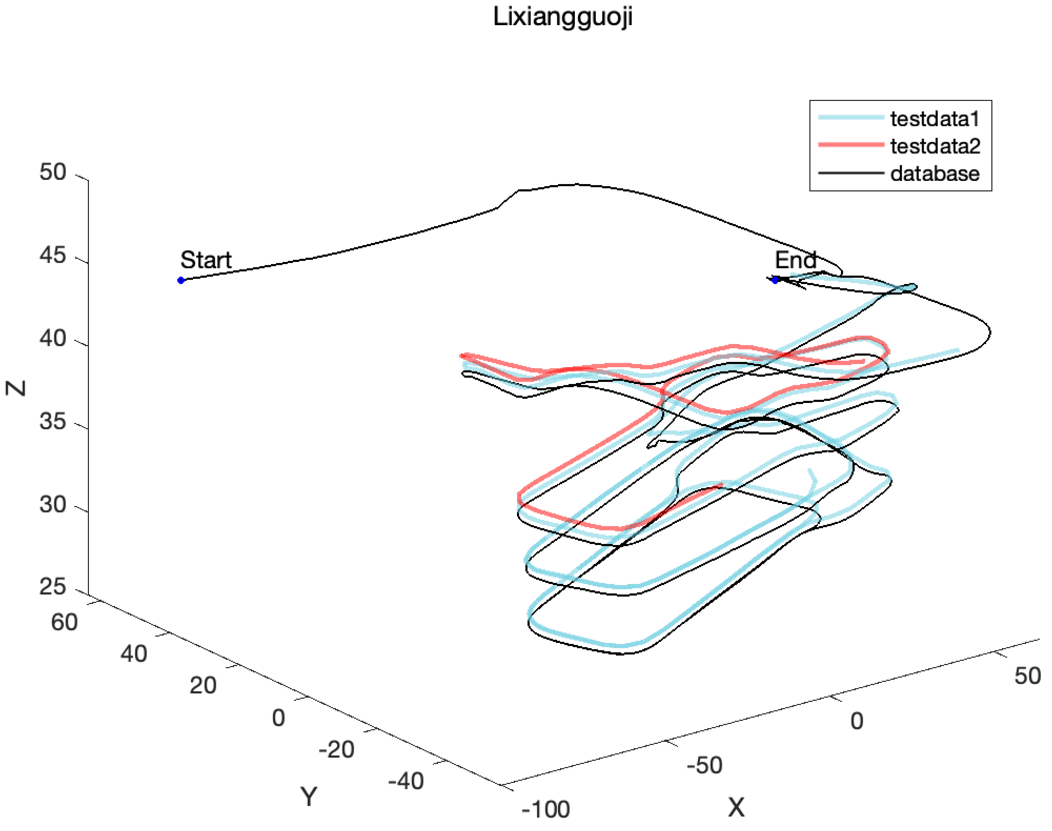
\includegraphics[width=0.24\textwidth]{Lixiangguoji.pdf}} 
    \subfigure[Yinwang]{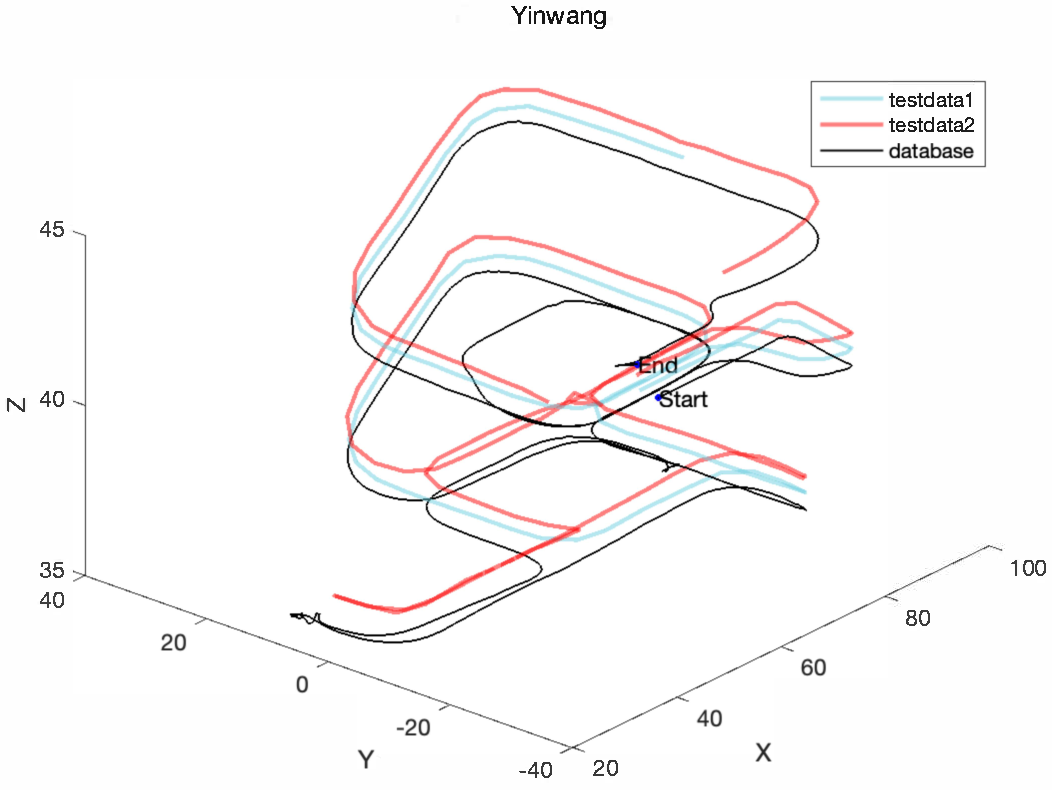
\includegraphics[width=0.24\textwidth]{Yinwang.pdf}}
    \subfigure[Yinzuo]{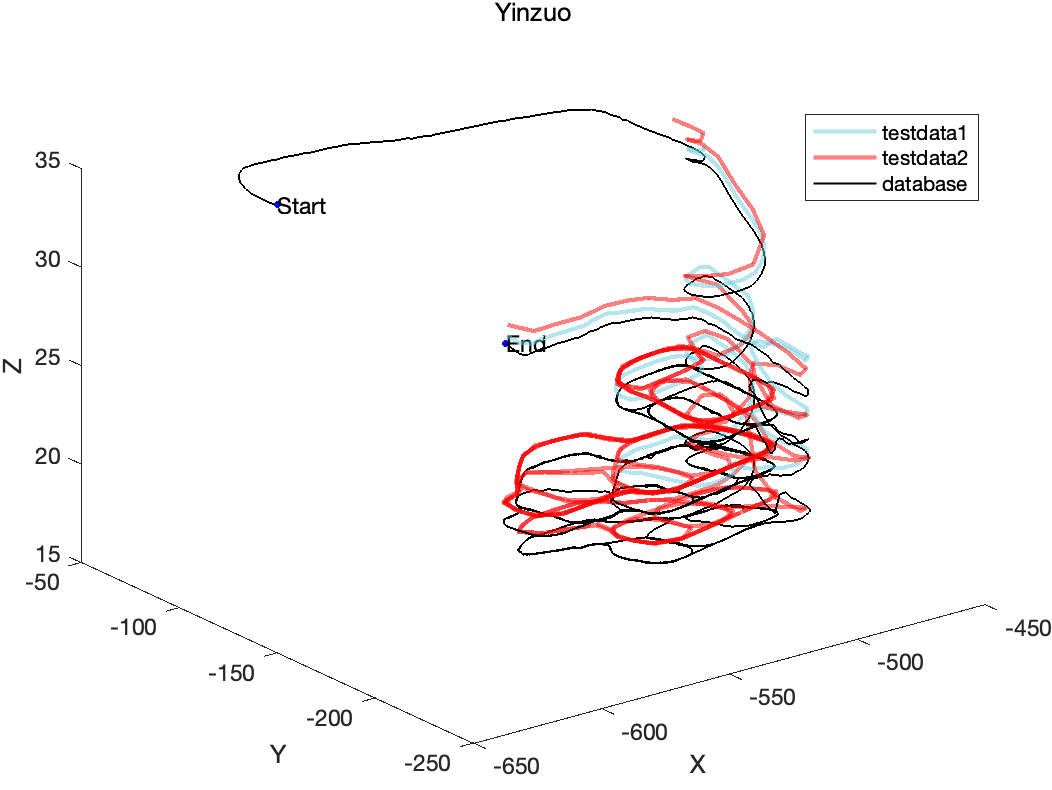
\includegraphics[width=0.24\textwidth]{Yinzuo.pdf}}
    \caption{\kevin{A visualization of trajectories of the experimental dataset. Each sub-figure has three trajectories of different colors, in which blue, red, and black represent the trajectories of test data 1, test data 2, and the database respectively. Trajectories of the same underground parking-lot were collected at different times over different days.}}
    \label{dataset}
    % \vspace{-0.18in}
\end{figure*}

\kevin{Once the NDT point cloud is obtained, our approach analyze each NDT cell by categorization of explicit geometric shape types, coupled with calculating the entropy of points within each NDT cell.}


\kevin{Our approach utilizes explicit categories to interpret the shape of each cell. For a given NDT cell, we calculate the sorted eigenvalues $e_1 > e_2 > e_3$ from the covariance matrix, together with their corresponding eigenvectors $v_1, v_2, v_3$. If $e_1 \gg e_2 \approx e_3$,  the shape of the cell will be classified as a straight line. Conversely, if $e_1 \approx e_2 \gg e_3$,  the cell will be considered a plane. However, this shape indicator requires two thresholds: 1) the ratio between $e_1$ and $e_2$, and 2) the ratio between $e_2$ and $e_3$. Instead of employing multiple thresholds, we propose an integrated one-dimensional NDT shape classification index:}
\begin{equation}
\label{g}
g=\frac{e_1\cdot e_3}{\left(e_2\right)^2}
\end{equation}
\kevin{Therefore, by employing a straightforward thresholding strategy on $g$, we can effectively classify the geometric shapes. As illustrated in Fig. \ref{g_figure}, $g$ enables the identification of four distinct shape categories: plane, ellipsoid, sphere, and line. To describe these explicit shape categories, we map the value of $g$ to different shapes using the following formula:}
\begin{equation}
    S = \left\{S \in \mathbb{Z}\ |\ S=\lceil \frac{g}{s} \rceil, 0\le g \le g_{max} \right\}
\end{equation}
\kevin{Here, $g_{\text{max}}$, $s$, and $S$ denote the maximum $g$ value selected, the segmented value we choose, and the geometric value, respectively.}
\kevin{Taking inspiration from NDD \cite{NDD}, we consider each NDT cell as a normal distribution characterized by a mean value $\mu$ and a covariance matrix $\Sigma$. Consequently, we utilize entropy, a statistical measure associated with the normal distribution, to describe the NDT cell:}
\begin{equation}
\label{entropy}
E=\frac{N}{2}(log2\pi+1)+\frac{1}{2} log\left| \Sigma \right|
\end{equation}
where $\left| \cdot \right|$ represents matrix determinant.

\kevin{Then, the Polar-Range-Height ROI partition $r$, $\theta$, $w$, geometric value $S$, and entropy $E$ of each NDT cell can be obtained. Due to the variance of spatial partition
between the voxel grid of NDT and ROI bins, it is likely that one ROI bin contains multiple NDT cells. The majority value of geometric values is used for $S$, and sum-pooling is applied for the entropy $E$.
The descriptor NDT-MC exclusively incorporates geometric value features, whereas NDT-MC-plus integrates both geometric value and entropy features.}

\subsection{Encoding}

% 地下停车场等室内环境的高度通常在3米左右。有用的信息主要分布在墙面、柱体等位置,但同时也存在来自车辆等动态物体的干扰。
% 这些动态物体的空间范围通常在0到2米之间。相比之下,室外环境的高度更高,同样也存在动态物体等干扰因素。

% 为了更好地进行地下停车场场景识别,我们希望给予停车位车辆上方空间更高的权重。
% 在室内环境中,其众多的结构化特征,例如:墙,柱等,提供的几何信息描述能力更强。
% 因此,我们仅使用前文中获取的几何值$S_{r,\theta,w}$,采用N+1进制编码来构建描述子NDT-MC。

% 在室外环境中,我们可以利用更多的高度信息。
% 然而,如果继续使用N+1进制编码,最高层处的权重将会变得非常大,使得整个描述子的性能主要由最高层所包含的信息决定。
% 为了使每个空间层级的权重更加合理即降低不同层之间的权重差,我们对N+1进制进行了对数映射。
% 此外,室外场景中存在许多非结构化场景,仅使用几何值$S_{r,\theta,w}$会降低我们的方法对室外场景的描述能力。
% 因此,为了增加整个描述子的区分性,我们使用熵$E_{r,\theta,w}$与几何值$S_{r,\theta,w}$一起构建描述子NDT-MC-plus。

\kevin{The maximum height of indoor environments is usually capped by a constant value (i.e. the height of the ceiling). Relevant patterns are repetitive, coupled with interference of dynamic objects. }
%walls, columns, and similar structures, but there is also interference from dynamic objects such as vehicles. The spatial range of these dynamic objects is usually between 0 and 2 meters. In comparison, outdoor environments have higher heights and also experience interference from dynamic objects.

%To improve the performance of indoor scenes, we aim to assign higher weight to the space above parking spaces. 
%In indoor environments, the numerous structured features, such as walls and columns, provide stronger geometric information. 
\kevin{To improve the performance, we only utilize the planar and cylinder shapes, denoted as $S_{r,\theta,w}$, with top-down-descending weights, and employ a base N+1 encoding to construct the descriptor NDT-MC.}

%In outdoor environments, we can leverage more height information. However, if we continue using the base N+1 encoding, the weight of the highest layer will become significantly large, making the overall performance of the descriptor primarily determined by the information contained in the highest layer. To ensure more reasonable weights for each spatial level and reduce the weight discrepancy between different layers, we apply a logarithmic mapping to the N+1 binary encoding. Additionally, outdoor scenes often involve many unstructured landmarks and relying solely on the geometric values, denoted as $S_{r,\theta,w}$, would diminish our method's descriptive ability for outdoor scenes. Therefore, to enhance the distinctiveness of the entire descriptor, we construct the descriptor NDT-MC-plus by combining the entropy, denoted as $E_{r,\theta,w}$, and the geometric values $S_{r,\theta,w}$.


\kevin{Given a polar coordinates index $\theta$ and a range-coordinate index $r$, the bin value $\mathcal{G}_{r,\theta}$, for each ROI, the NDT-MC can be calculated by:}
\begin{equation}
    \label{mathcal_L_r}
    \mathcal{L}_{r,\theta}=\sum_{w=0}^{N_z}{\left(N+1\right)^w\cdot}S_{r,\theta,w}
\end{equation}
\kevin{, where $N_z$ represents the number of selected height layers, and $N$ is the number of chosen NDT shapes.} 
\kevin{To leverage the variety of landmarks for on-road driving, we propose NDT-MC-plus by a combination of the geometric values $S_{r,\theta,w}$ and the entropy $E_{r,\theta,w}$. 
Similarly, NDT-MC-plus can be obtained by calculating $\mathcal{G}$ and $\mathcal{E}$ for each ROI:}
\begin{equation}
    \mathcal{G}_{r,\theta}=\sum_{w=0}^{N_z}{\left(w+1\right)\cdot}S_{r,\theta,w}
    \label{eq:11}
\end{equation}
\begin{equation}
    \label{mathcal_E_r}
    \mathcal{E}_{r,\theta}=\sum_{w=0}^{N_z}{\left(w+1\right)\cdot}E_{r,\theta,w}
\end{equation}

\kevin{Note, for outdoor scenes, we apply a logarithmic mapping to the base N+1 encoding in Eq. \ref{eq:11} to balance the weights of different layers.}
 %By applying Eq. \ref{mathcal_L_r} to all polar-range coordinate bins, we obtain the final NDT-MC global descriptor. Similarly, by applying Eq. \ref{mathcal_G_r} and Eq. \ref{mathcal_E_r} to all polar-range coordinate bins, we obtain the final NDT-MC-plus global descriptor.

\section{DESCRIPTORS MATCHING}

\subsection{Fast Matching}

% 描述子数据库规模随着机器人所探索区域的增大而逐渐增加,机器人需要花费更多的时间对当前描述子与数据库中描述子进行匹配,这将会影响整个回环检测过程的效率。为了实现快速描述子检索,迫切需要一种高效的算法。

% \textbf{geometric key(GK)的构建}。为了解决完整描述子构建和检索的计算成本高的问题,我们提出了一种基于Histogram的Key叫做geometric key。如Fig. \ref{GK}所示,在通过Eq. \ref{g}计算出一帧NDT Point Cloud中所有NDT Cells的g值之后,我们按照g值所属的值域将其投入对应列中即所在列的值加1,最终得到一个$1×N_s$的向量,其中$N_s$表示一个所选用的几何值$S$最大值。

% \textbf{基于KD-Tree的快速检索}。直接采用完整描述子构造KD-Tree和检索所需要的计算负荷大,其时间复杂度分别为 $O(n2N_r N_{\theta} log⁡(n))$ 和 $O(n^{(1-1/2N_r N_θ )})$ ,其中 $n$ 表示描述子的数量。我们的GK的维度为$1×N_s$,且$N_s$在本文中小于$N_r$和$N_θ$,因此采用GK构造KD-Tree进行快速检索,这样在构造KD-Tree的过程中时间复杂度为$O(n2N_s log⁡(n))$。

% 在完成GK KD-Tree的构造之后,我们进一步进行K最近邻搜索。通过在已构建的KD Tree中搜索查询GK,我们可以获得与查询相关的K个最近邻的候选帧。

% \textbf{自适应距离判断}。在SC-LIO-SAM\footnote{https://github.com/gisbi-kim/SC-LIO-SAM}中,会通过对K最近邻搜索进行完整描述子即Scan Context的匹配,最后选择出一个相似度距离最小的候选帧作后续阈值判断以选取最终的描述子。然而,在SLAM系统所提供的每一帧的位姿估计能够有效的作为先验信息对K个最近邻的候选帧进行判断,即对其进行距离阈值的判断以进一步筛选候选帧。考虑到SLAM轨迹存在一个随着时间/距离增长而增加的累积误差,为了能够更好的检测回环,我们采用我们之前的方法\cite{opscf}所提出的自适应欧式距离阈值:
% \begin{equation}
% r=30+N_{keyframe}/n_o
% \end{equation}
% 其中$N_{keyframe}$是当前关键帧的数量,$n_o$是里程计的累积误差的设计参数,其具体的值取决于所采用的里程计。

% \textbf{Sector Key的构建}。如果候选关键帧满足自适应距离阈值,那么将候选帧的描述子与当前帧描述子进行相似度距离阈值判断。正如前文中所言,我们可以通过列位移实现描述子的旋转不变性,然而对所有列的位移必然会导致计算复杂度的增加。我们采用与Scan Context相同的方式,对描述子按列求均值得到一个$1×N_{\theta}$的向量Sector Key。通过对两帧描述子的Sector Key进行列位移计算相似度距离,得出一个大致的列位移量。再对该列位移附近位移区域进行描述子匹配获得相似度距离值。

\textbf{Construction of geometric key (GK)}: \kevin{Instead of using complete descriptors, we propose a histogram-based key called \emph{geometric key}, to reduce the computation in similarity matching of descriptors. 
%As shown in Fig. \ref{GK}, after calculating the $g$ values for all NDT cells in a frame's NDT representation using Eq. \ref{g}, we distribute them into corresponding columns according to their value ranges. 
As shown in Fig. \ref{GK}, we discrete the continuous $g$ values of NDT representations into columns with an increment of 1. This process results in a $1 \times N_s$ vector, where $N_s$ represents the maximum value of the selected geometric value $S$.}

\textbf{Fast Retrieval based on kd-tree}: 
\kevin{By using the geometry key, the time complexity of kd-tree construction can be reduced from $O(n2N_r N_{\theta} \log(n))$ to $O(n2N_s \log(n))$, given the size of geometry $N_s$ is much smaller than both $N_r$ and $N_{\theta}$.}
%Constructing and retrieving a kd-tree directly from complete descriptors incurs a high computational load, with time complexities of $O(n2N_r N_{\theta} \log(n))$ and $O(n^{(1-1/2N_r N_{\theta} )})$ respectively, where $n$ denotes the number of descriptors. Since the dimension of our geometry key is $1 \times N_s$, and $N_s$ is smaller than both $N_r$ and $N_{\theta}$ in this paper, we use the geometry key to construct a kd-tree for fast retrieval. This approach reduces the time complexity to $O(n2N_s \log(n))$ during the kd-tree construction process.
\kevin{Once the kd-tree is built, we undergo the k-nearest neighbor search for each query. }

\textbf{Adaptive distance threshold}: 
SLAM systems are able to provide pose estimation. After $k$ candidate frames are obtained, the candidate frames are further filtered by applying distance threshold judgment. With the consideration of the cumulative error increasing over time and distance in SLAM trajectories, we employ adaptive Euclidean distance thresholding used in our previous method \cite{opscf}.
% In SC-LIO-SAM\footnote{https://github.com/gisbi-kim/SC-LIO-SAM}, complete descriptor matching, specifically Scan Context, is performed through k-nearest neighbor search. The frame with the smallest similarity distance among the K candidates is selected for subsequent threshold-based judgment to determine the final descriptor. However, the pose estimation provided by the SLAM system for each frame can effectively serve as prior information for judging the K candidate frames, i.e., by applying a distance threshold judgement to further filter the candidate frames. With the consideration of the cumulative error increasing over time and distance in SLAM trajectories, we employ an adaptive $Euclidean$ distance thresholding used in our previous method \cite{opscf}.


\textbf{Construction of Sector Key}: If a candidate keyframe satisfies the adaptive distance threshold, \kevin{we compare its descriptor with that of the current frame using a similarity score. As mentioned earlier, rotation invariance is achieved by performing column shifts. However, iterating all columns will inevitably increase the computational complexity. Following $Scan Context$, we compute the column-wise average of the descriptor to obtain a $1 \times N_{\theta}$ vector called the \emph{sector key}.
Sector keys simplify column shift approximation calculation, and descriptor matching is performed in the vicinity of the estimated column shift.}

\subsection{Descriptors matching}

% 我们的描述子NDT-MC和NDT-MC-plus采用cosine distance和correlation coefficient对描述子之间的相似度距离进行计算。
\kevin{Our approach uses correlation coefficient as the similarity metric.}

\kevin{Given two descriptors $D_q=\left\{c_q^0,\ c_q^1,\ldots,c_q^{N_\theta}\right\}$, $D_c=\left\{c_c^0,\ c_c^1,\ldots,c_c^{N_\theta}\right\}$, $c_q^i$ and $c_c^i$ represent the $i^{th}$ column of $D_q$ and $D_c$ respectively. }

\kevin{Given a query descriptor $D_q$ to $\left\{c_q^0,\ c_q^1,\ldots,c_q^{N_\theta},c_q^0,\ c_q^1,\ldots,c_q^{N_ \theta-1}\right\}$,} The calculation method of correlation coefficient between the two descriptors is:
\begin{equation}
g_k\left(D_q^k,D_c\right)=1-\frac{1}{N_\theta+1}\sum_{i=0}^{N_\theta}\left(\frac{(c_q^{i+k}-\overline Q) \cdot (c_c^i - \overline C )}{{\Vert c_q^{i+k} - \overline Q \Vert}\cdot{\Vert c_c^i - \overline C \Vert}}\right)
\label{calculate correlation similirity distance}
\end{equation}
Where $\overline C$ and $\overline Q$ represent the mean of all elements of $D_c$ and $D_q^k$ respectively.

\kevin{Then, column-shifting is employed to find the appropriate yaw angle to match:}
\begin{gather}
g_s\left(D_q,D_c\right)=min\left(g_k\left(D_q^k,D_c\right)\right) \label{g_s} \\
k\in\left\{0,1,\ldots,N_\theta-1\right\}
\label{calculate maximum similirity}
\end{gather}
\kevin{where $D_q^k$ means $D_q$ shifted by $k^{th}$. We determine the similarity between two frame descriptors by calculating the minimum similarity obtained through column displacement.}

\section{EXPERIMENT EVALUATION}

% \begin{table*}
% \centering
% \caption{Comparison of the Top 1 Recall results of the five methods in the test data of 8 underground parking lots}
% \label{table2}
% \arrayrulecolor{black}
% \tiny
% \resizebox{0.98\linewidth}{!}{
% \begin{tabular}{c|l|c|c|c|c|c|c|c|c} 
% \hline
% \multicolumn{2}{c|}{\multirow{2}{*}{Database}} & \multicolumn{8}{c}{Top 1 Recall Rate(\%)}                                                               \\ 
% \cline{3-10}
% \multicolumn{2}{c|}{}                          & \multicolumn{1}{l|}{Ours 2m} & Ours 1m       & SC 2m & SC 1m         & Iris 2m & NetVLAD & NDT-Hist 2m  & NDD\\ 
% \hline
% \multirow{2}{*}{Rongke}        & Test data 1   & \textbf{77.0}                & 71.5          & 36.7  & 46.7          & 47.4    & 53.1    & 5.2   &    37.7    \\ 
% \cline{2-10}
%                                & Test data 2   & \textbf{77.6}                & 61.9          & 21.0  & 23.1          & 60.2    & 17.1    & 5.1   &  23.4     \\ 
% \hline
% \multirow{2}{*}{Lixiangguoji}  & Test data 1   & 89.4                         & \textbf{94.1} & 81.3  & 92.3          & 85.8    & 34.1    & 22.3    &   82.5  \\ 
% \cline{2-10}
%                                & Test data 2   & \textbf{94.5}                & 92.3          & 71.4  & 91.2          & 81.3    & 72.5    & 18.7  & 71.7       \\ 
% \hline
% \multirow{2}{*}{Yinwang} & Test data 1   & \textbf{95.7}                & \textbf{95.7} & 59.6  & \textbf{95.7} & 61.7    & 83.0    & 17.0     & 84.2    \\ 
% \cline{2-10}
%                                & Test data 2   & 97.9                         & \textbf{98.6} & 74.6  & 95.1          & 80.3    & 52.1    & 12.0 & 62.0        \\ 
% \hline
% \multirow{2}{*}{Yinzuo}        & Test data 1   & 91.7                         & \textbf{94.4} & 35.4  & 81.9          & 63.2    & 63.2    & 14.6     & 57.6    \\ 
% \cline{2-10}
%                                & Test data 2   & 95.8                         & \textbf{97.4} & 81.1  & 95.6          & 82.2    & 73.6    & 20.3 & 83.8        \\ 
% \hline
% \multicolumn{2}{c|}{Overall}                   & \textbf{86.9}                & 84.0          & 54.6  & 69.3          & 68.6    & 45.9    & 13.2  & 58.1       \\
% \hline
% \end{tabular}
% }
% \end{table*}

\begin{table*}
    \centering
    \caption{\kevin{The comparison of the top-1 recall among the five methods in the test data of 8 underground parking lots.}}
    \label{table2}
    \arrayrulecolor{black}
    \tiny
    \resizebox{0.98\linewidth}{!}{
    \begin{tabular}{c|l|c|c|c|c|c|c} 
    \hline
    \multicolumn{2}{c|}{\multirow{2}{*}{Database}} & \multicolumn{6}{c}{Top 1 Recall Rate(\%)}                                                               \\ 
    \cline{3-8}
    \multicolumn{2}{c|}{}                          & \multicolumn{1}{l|}{NDT-MC 2m}  & SC 2m & Iris 2m & NetVLAD & NDT-Hist 2m  & NDD\\ 
    \hline
    \multirow{2}{*}{Rongke}        & Test data 1   & \textbf{77.0} & 36.7  & 47.4    & 53.1    & 5.2   &    37.7    \\ 
    \cline{2-8}
                                   & Test data 2   & \textbf{77.6} & 21.0 & 60.2    & 17.1    & 5.1   &  23.4     \\ 
    \hline
    \multirow{2}{*}{Lixiangguoji}  & Test data 1   & \textbf{89.4}  & 81.3    & 85.8    & 34.1    & 22.3    &   82.5  \\ 
    \cline{2-8}
                                   & Test data 2   & \textbf{94.5} & 71.4 & 81.3    & 72.5    & 18.7  & 71.7       \\ 
    \hline
    \multirow{2}{*}{Yinwang} & Test data 1   & \textbf{95.7} & 59.6  & 61.7    & 83.0    & 17.0     & 84.2    \\ 
    \cline{2-8}
                                   & Test data 2   & \textbf{97.9} & 74.6 & 80.3    & 52.1    & 12.0 & 62.0        \\ 
    \hline
    \multirow{2}{*}{Yinzuo}        & Test data 1   & \textbf{91.7} & 35.4 & 63.2    & 63.2    & 14.6     & 57.6    \\ 
    \cline{2-8}
                                   & Test data 2   & \textbf{95.8} & 81.1 & 82.2    & 73.6    & 20.3 & 83.8        \\ 
    \hline
    \multicolumn{2}{c|}{Overall}                   & \textbf{86.9}   & 54.6  & 68.6    & 45.9    & 13.2  & 58.1       \\
    \hline
    \end{tabular}
    }
    \end{table*}

\begin{figure*}[t]
 \centering  %居中
 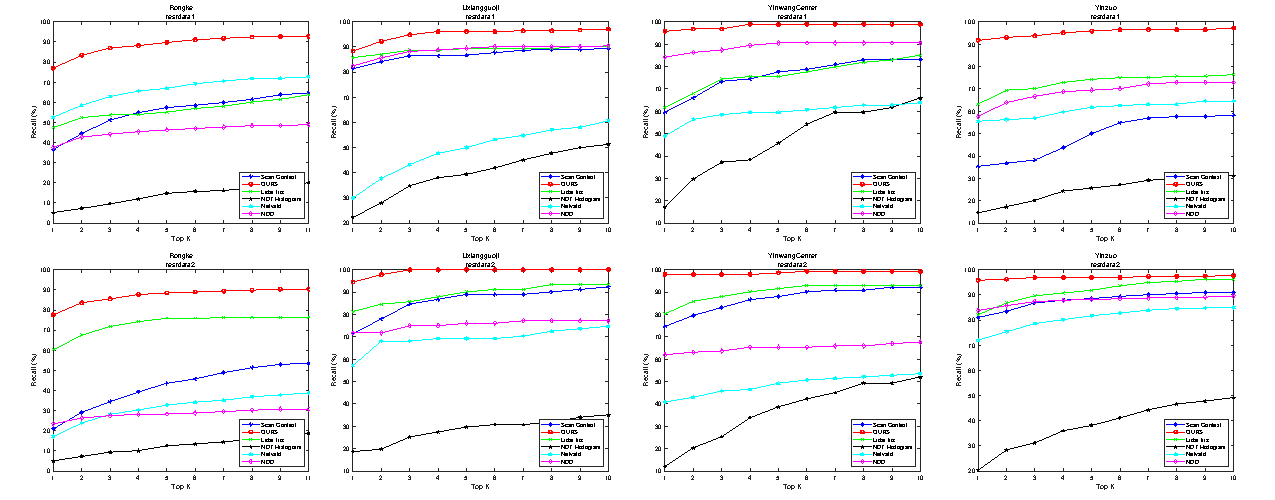
\includegraphics[width=1\linewidth,height=6cm]{topkrecall_new.pdf} 
 %scale为图片大小的缩放比例 res3为图片名
 %设置图像的描述(会自动生成编号)
 \caption{\kevin{The top-k recall rate curves of NDT-MC, Scan Context, NetVLAD, NDT-Histograms and Lidar Iris in four underground parking-lots experiments. The values of $k$ ranging from 1 to 10 are investigated.}}
 \label{topkrecall}
 % \vspace{-0.18in} %
\end{figure*}


\begin{table*}
\centering
\caption{The comparison of the F1 score and extended precision results on the KITTI dataset.}
\label{f1score}
\tiny
\resizebox{0.98\linewidth}{!}{
\begin{tabular}{c|c|c|c|c|c|c}
\hline
Method & 00 & 02 & 05 & 06 & 07 & 08 \\
\hline
SC & 0.924/0.891 & 0.690/0.516 & 0.859/0.902 & 0.932/0.982 & 0.482/0.630 & 0.608/0.667 \\
\hline
ISC & 0.856/0.737 & 0.675/0.510 & 0.847/0.813 & 0.937/0.921 & 0.506/0.634 & 0.719/0.710 \\
\hline
IRIS & 0.873/0.909 & 0.813/\textbf{0.860} & 0.922/0.925 & 0.936/0.971 & 0.585/0.710 & 0.534/0.665 \\
\hline
M2DP & 0.885/0.911 & 0.616/0.500 & 0.802/0.799 & 0.945/0.920 & 0.515/0.589 & 0.022/0.500 \\
\hline
PointNetVlad & 0.779/0.641 & 0.727/0.691 & 0.541/0.536 & 0.852/0.767 & 0.531/0.591 & 0.037/0.500 \\
\hline
NDD & 0.943/\textbf{0.963} & 0.851/0.592 & 0.947/0.941 & 0.989/0.976 & \textbf{0.659}/\textbf{0.713} & \textbf{0.851}/0.661 \\
\hline
NDT-MC & 0.911/0.858 & 0.8/0.54 & 0.927/0.911 & 0.989/0.983 & 0.534/0.652 & 0.49/0.541 \\
\hline
NDT-MC-plus & \textbf{0.954}/0.942 & \textbf{0.871}/0.854 & \textbf{0.952}/\textbf{0.949} & \textbf{0.993}/\textbf{0.993} & 0.615/\textbf{0.713} & 0.736/\textbf{0.752} \\
\hline
\end{tabular}
}
\end{table*}


% PR-Curve看不出明显的优势,可以注释掉。
% \begin{figure*}[htbp]
% \centering
% \begin{tabular}{ccc}
% \subfigure[KITTI 00]{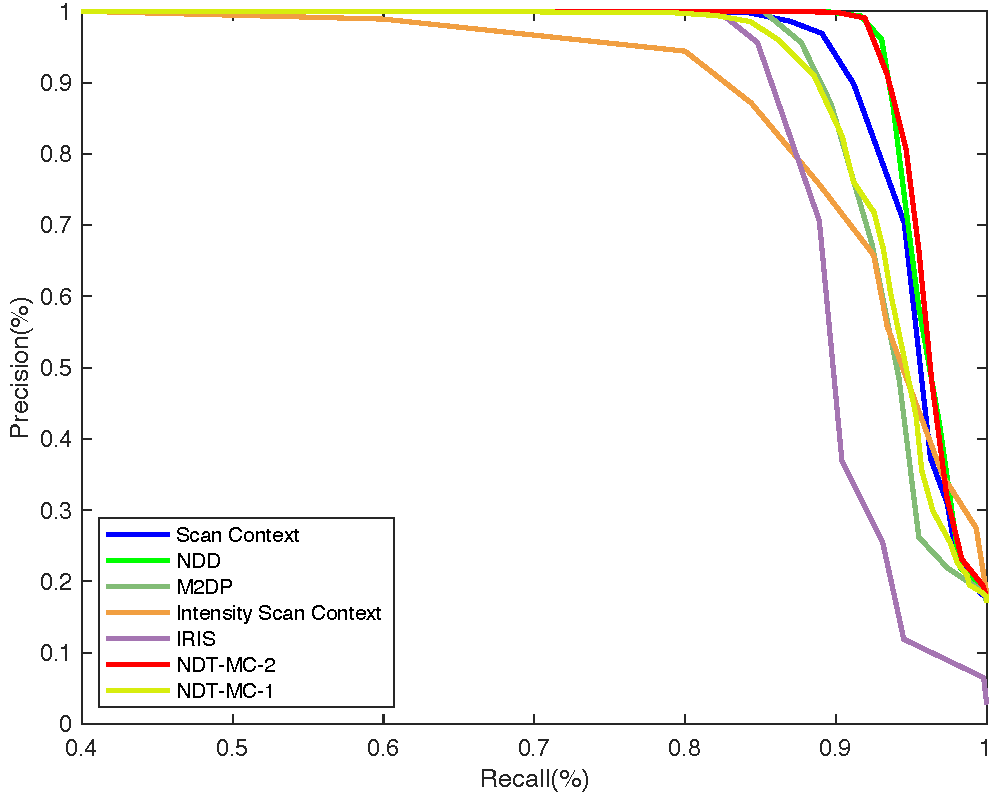
\includegraphics[width=0.33\textwidth]{./figure/PRCurve/KITTI00.pdf}} &
% \subfigure[KITTI 02]{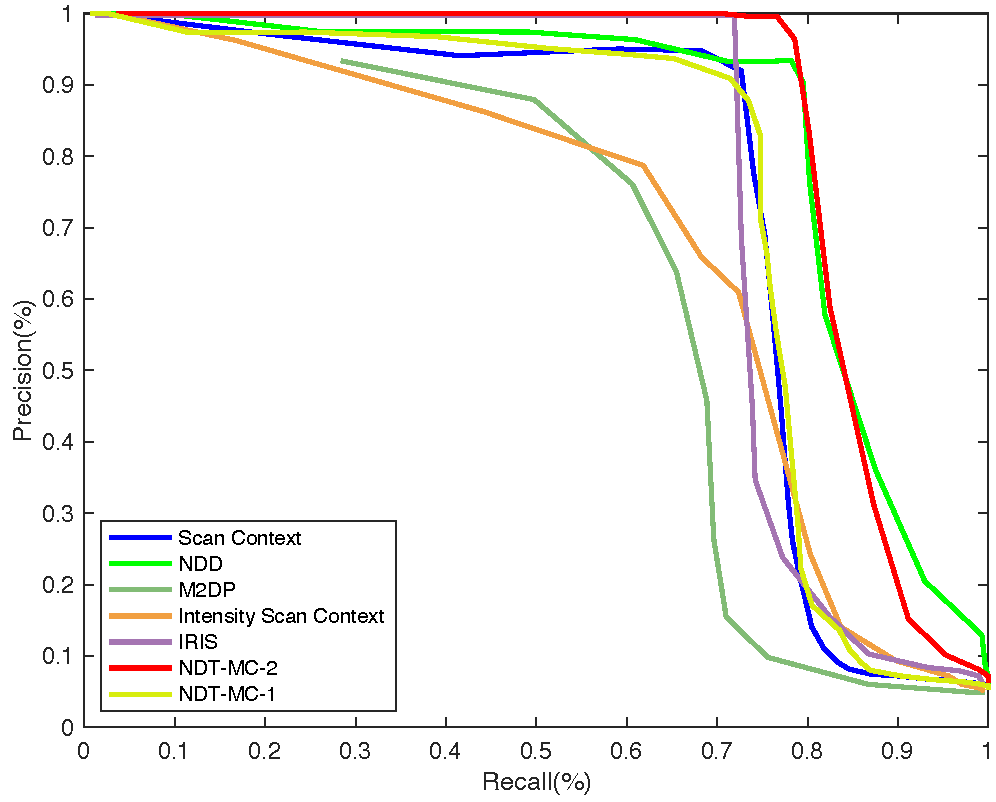
\includegraphics[width=0.33\textwidth]{./figure/PRCurve/KITTI02.pdf}} &
% \subfigure[KITTI 05]{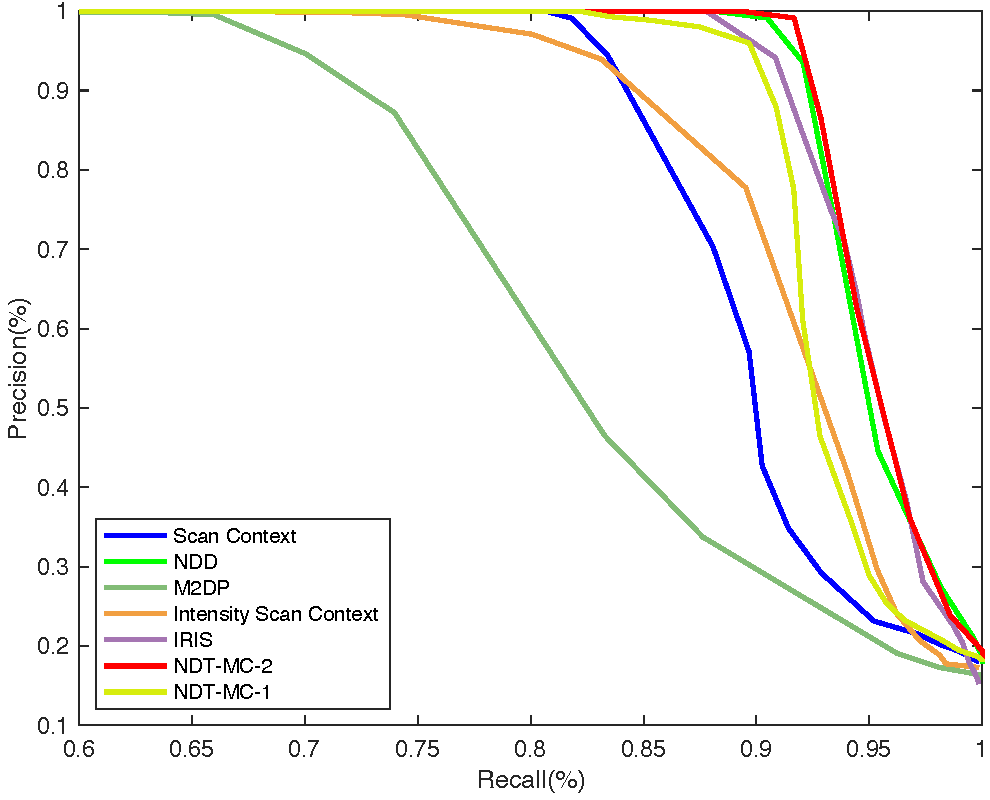
\includegraphics[width=0.33\textwidth]{./figure/PRCurve/KITTI05.pdf}} \\
% \subfigure[KITTI 06]{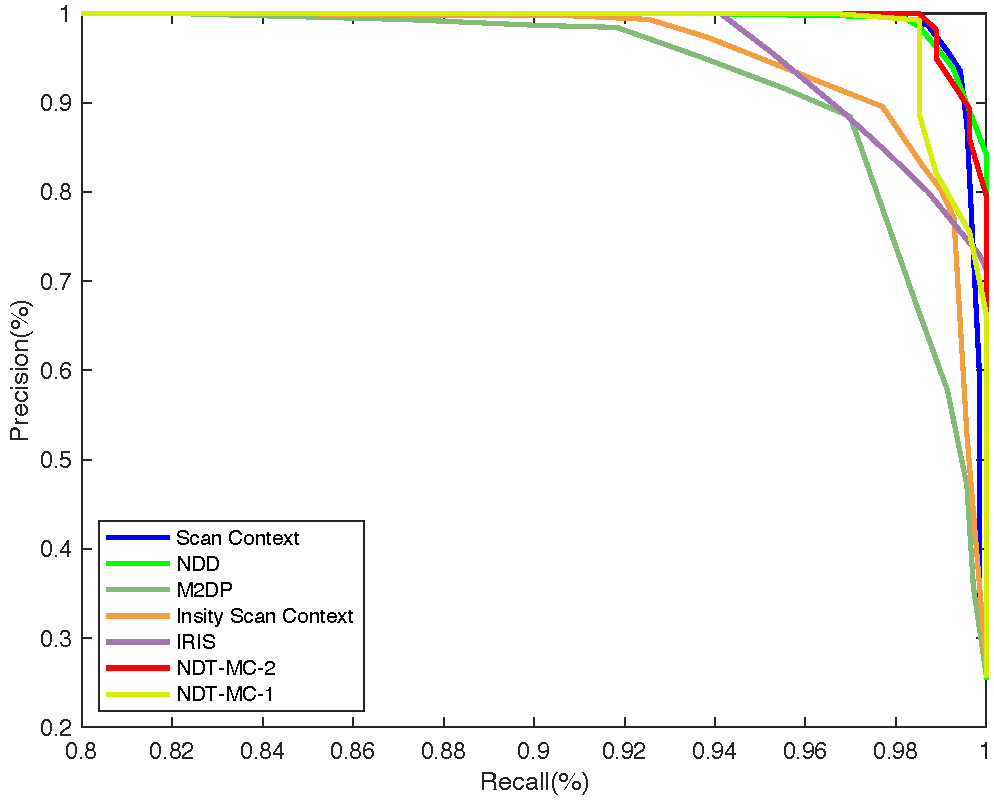
\includegraphics[width=0.33\textwidth]{./figure/PRCurve/KITTI06.pdf}} &
% \subfigure[KITTI 07]{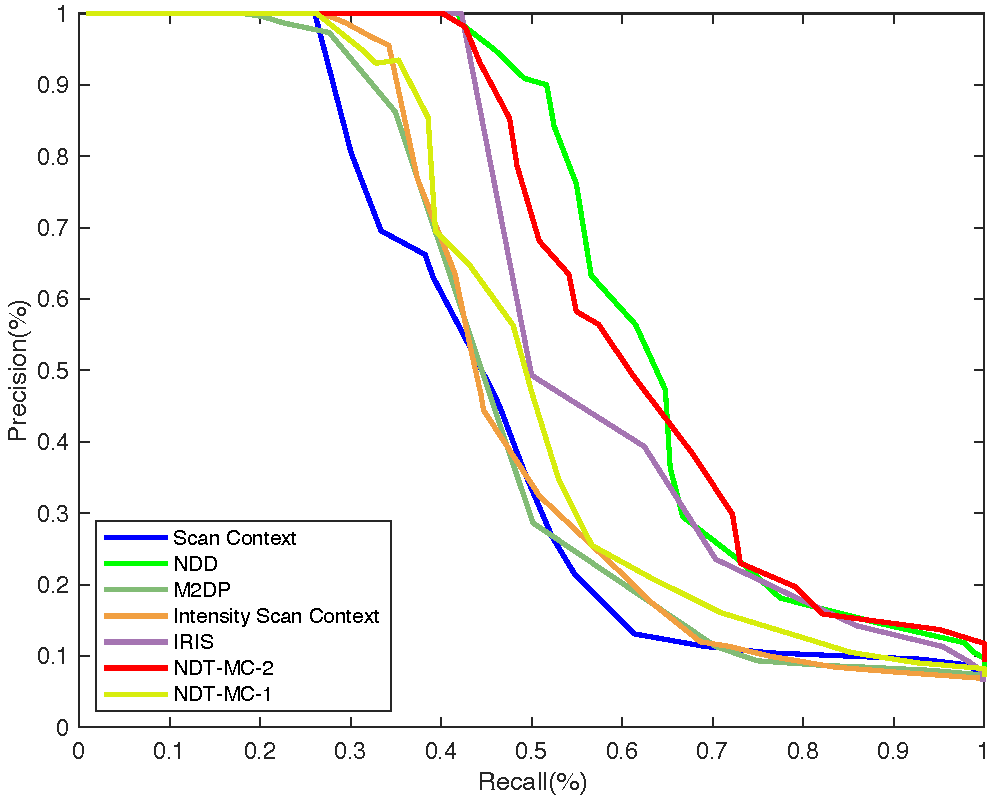
\includegraphics[width=0.33\textwidth]{./figure/PRCurve/KITTI07.pdf}} &
% \subfigure[KITTI 08]{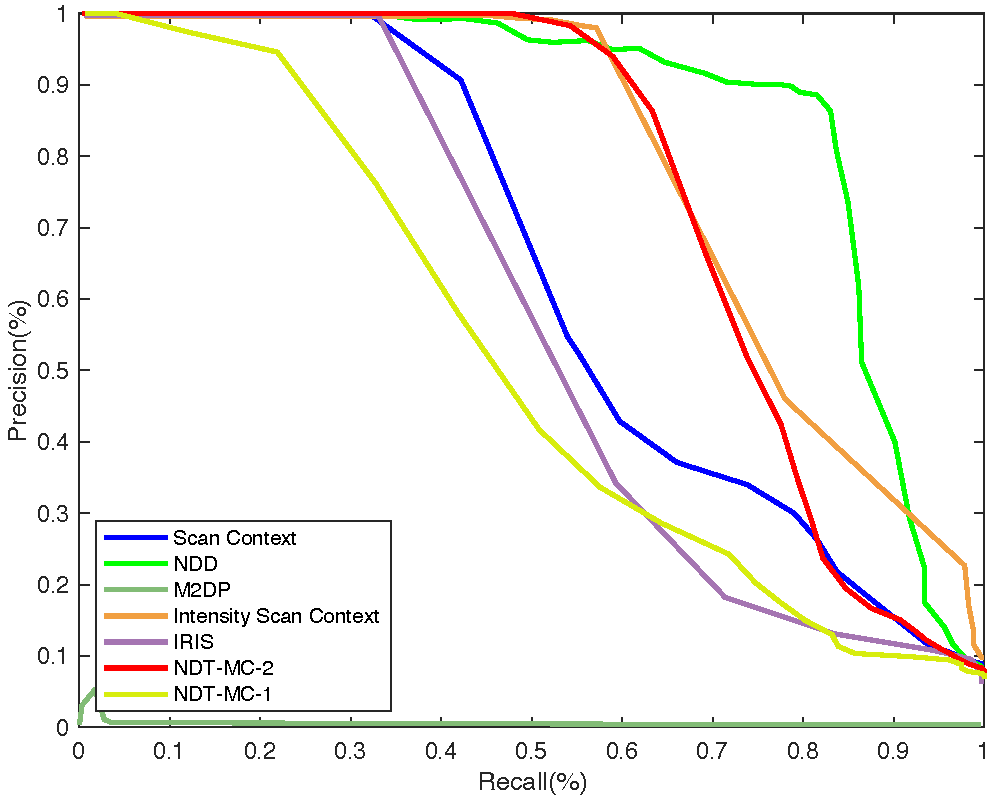
\includegraphics[width=0.33\textwidth]{./figure/PRCurve/KITTI08.pdf}}
% \end{tabular}
% \caption{Precision-Recall Curve}
% \label{prcurve}
% \end{figure*}

\begin{figure}
	\centering
	\subfigure[NDT-MC-plus-LIO-SAM]{
		\begin{minipage}{8cm} %[b]%{0.2\textwidth} 
                        %{12cm or 0.2/textwidth} 控制图片大小,可以=textwidth
			% 插入子图片
                        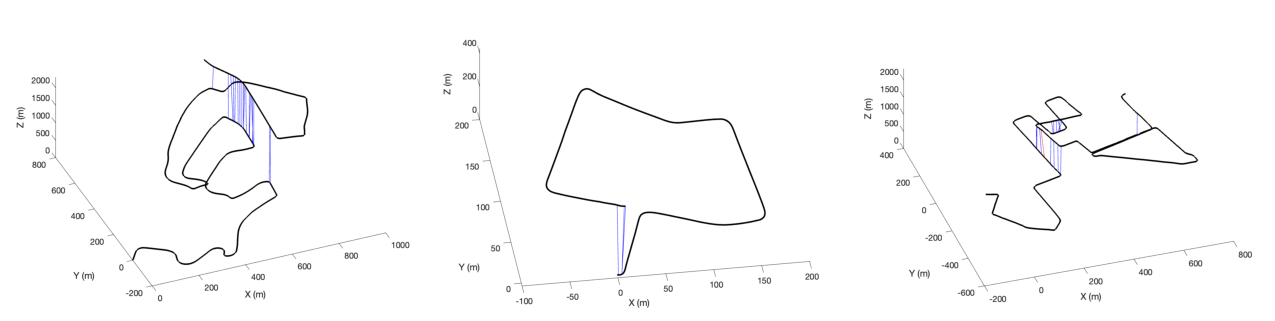
\includegraphics[width=\textwidth]{ndtmc-liosam.pdf} \\
			%\includegraphics[width=\textwidth]{fig/beforePAA.eps} 
                        % 可以在一个minipage里写多张图片,它们共用一个小标题\subfigure['sub_title']
		\end{minipage}
	}
% 百度里有个方法说这里要空格,但我不空格也是上下排版的,疑惑
	\subfigure[SC-LIO-SAM]{
		\begin{minipage}{8cm}%[b]%{0.2\textwidth}
			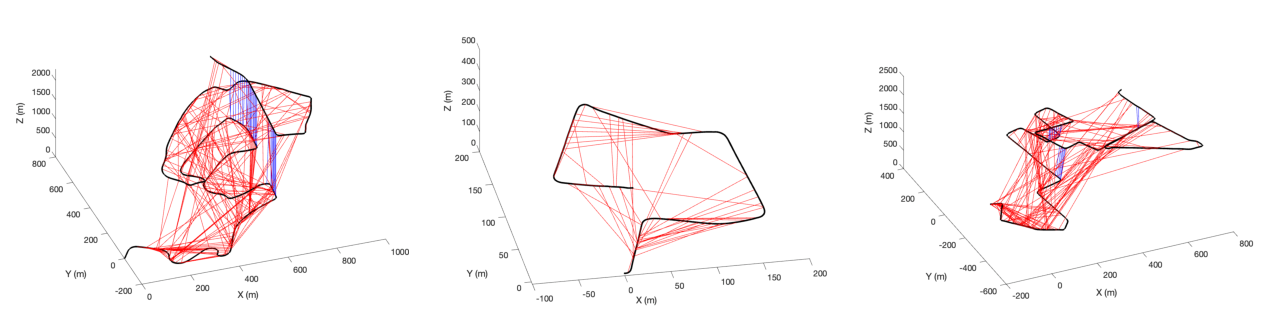
\includegraphics[width=\textwidth]{sc-liosam.pdf} \\
			
		\end{minipage}
	}
    \caption{\kevin{The visualization of true/false positive matches for KITTI sequence 02, 07, and 08. Blue and red represent correct and incorrect loop closures, respectively.}} 
	\label{T/FMatch}
\end{figure}

\begin{figure}[t]
    \centering  %居中
    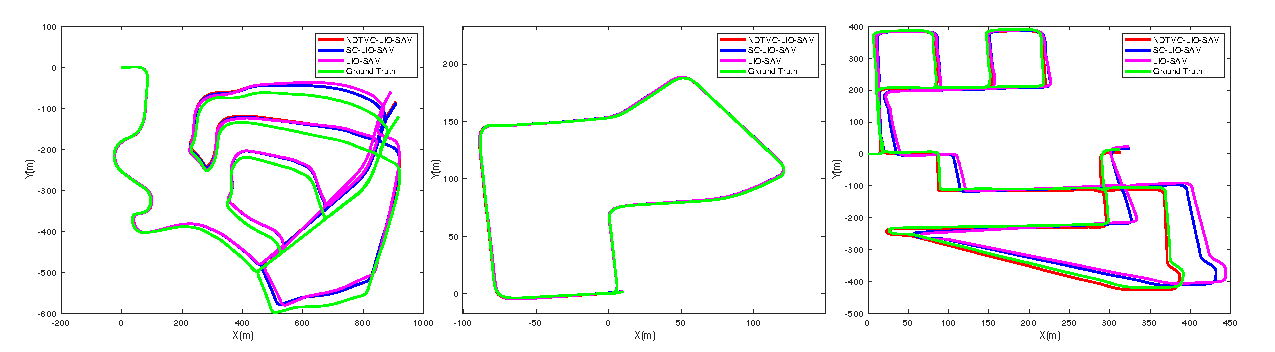
\includegraphics[width=\linewidth]{trajectorycompare.pdf} 
    %scale为图片大小的缩放比例 res3为图片名
    %设置图像的描述(会自动生成编号)
    \caption{\kevin{The comparison of trajectories on KITTI sequence 02, 07 and 08. The trajectories of NDTMC-LIO-SAM, SC-LIO-SAM, LIO-SAM, and ground truth are represented in red, blue, rose red, and green, respectively.}}
    \label{trajectorycompare}
    \vspace{-0.18in} %
\end{figure}

\begin{figure}[t]
    \centering  %居中
    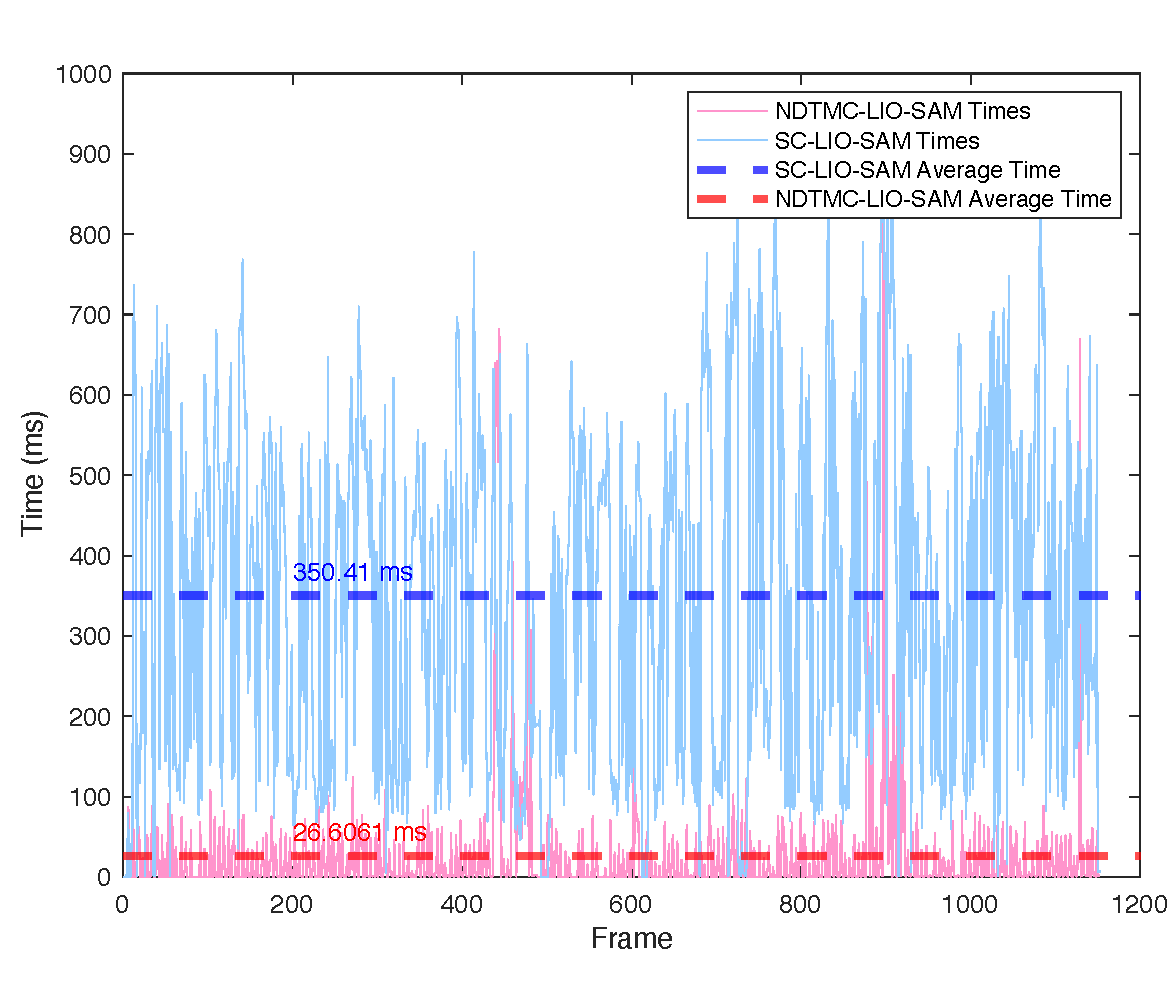
\includegraphics[width=\linewidth,height=5cm]{timecompare.pdf} 
    %scale为图片大小的缩放比例 res3为图片名
    %设置图像的描述(会自动生成编号)
    \caption{\kevin{The algorithm run-time latency. The red and blue lines represent the run-time latency required by the NDTMC-plus-LIOSAM and SC-LIO-SAM methods, respectively, for each frame's loop closure detection on KITTI sequences 02, 07, and 08. The red and blue dashed lines indicate the average time latency required by these two methods.}}
    \label{timecompare}
    \vspace{-0.18in} %
\end{figure}



\subsection{Dataset for experiments}

\kevin{Our experiments have two distinct scenarios. We collect a dataset for underground parking lots localization (NIO underground parking-lot dataset), while the widely-used KITTI dataset\cite{KITTI} is also used for the evaluation of loop closure detection for on-road driving.}

\textbf{NIO underground parking-lot dataset.} \kevin{This dataset is collected in real-world underground parking lots using a robocar equipped with a hybrid mechanical lidar (that of a FoV of $ 120^{\circ} \times 25^{\circ}$). As shown in Fig. \ref{dataset}, the dataset consists of four different parking lots, located in the basements of four commercial malls, i.e. Rongke, Lixiangguoji, Yinwang, and Yinzuo. Multi-session data is collected at each site, and multi-session SLAM is used to obtain globally-consistent trajectories and point cloud maps. 
A place is defined as a submap built by a trajectory segment of 4m. 
For each underground parking lot, the session with the largest map area (with the largest number of places), is selected as the database. Other sessions are used for testing. Because the pipeline is designed for crowd-sourced mapping, NDT representation is used instead of raw point cloud map. If the distance between the query pose and database pose is within the range of 4m on the x-y plane and 2m on the z-axis to a database pose, it will be considered as a true positive pair.} The numbers of loop closures in test data 1 and test data 2 at Rongke are 439 and 415 respectively. Similarly, the numbers of loop closures at Lixiangguoji, Yinwang, and Yinzuo are 310 and 91, 94 and 142, 144 and 454.
\kevin{In Fig. \ref{dataset}, the database and testing trajectories of the four experiments are shown.}

\textbf{KITTI dataset.} \kevin{The sequence data in the KITTI dataset is used for this evaluation, where point cloud data is acquired using the Velodyne HDL-64E lidar sensor. Our experiment follows the same setting with NDD \cite{NDD}.}
%For our research,  six sequences, i.e. sequences 00, 02, 05, 06, 07, and 08 are used.
%Among these sequences, sequence 08 exclusively includes a loop path in the reverse direction. On the other hand, sequence 02 encompasses loops in various directions. As for sequences 00, 05, 06, and 07, they all consist of loops in the same direction. 

\subsection{Experimental settings}

\textbf{Experiment on NIO underground parking-lot dataset.} \kevin{In this experiment, the observation point cloud is a local map within an 80-meter trajectory built by lidar-inertial odometry. The observation is converted to NDT for global descriptor extraction. The database is built from submaps cropped on the global NDT map. Each query observation is guaranteed to find its true positive location in the database. For each query observation, Eq. \ref{calculate correlation similirity distance} and Eq. \ref{g_s} are used to retrieve the most similar location from the database. A successful place recognition will be considered if the retrieved x-y location is within 4m and z location is within 2m of the query, otherwise, a failure localization.}

\kevin{The proposed method is evaluated on eight testing datasets collected in four underground parking lots. For comparison, state-of-the-art place recognition methods are implemented, i.e., Scan Context\cite{kim2018scan}, Lidar Iris\cite{wang2020lidar}, NetVLAD\cite{arandjelovic2016netvlad}, NDD\cite{NDD} and NDT-Histograms\cite{ndt_histograms}. Due to the fact that Scan Context-like methods are not designed for underground parking lots, we make the following adaptations: points below 2m w.r.t. lidar coordinate system are used for descriptor representation. For Scan Context and Lidar Iris, NDT Submap is cropped according to vehicle poses as the input. For NetVLAD, front wide-angle images are used. For a fair comparison, the proposed method, Scan Context, and Lidar Iris are set with the same parameters, i.e., $N_r$=40, $N_\theta$=60, $Z$=3m, $L_z$=1m and $R$=80m. Since NDD requires the raw point cloud as input, both the observation and the database use the raw point cloud submap stitched by LIO. The top $n$ recall rate is used as the main evaluation metric.}

\textbf{Experiment on KITTI.} \kevin{In this experiment, we define a true positive detection if the distance between the query and matched database frame node is less 5 meters. Note, consecutive frames within a certain range will not be considered as positive pair.}
% KITTI数据集符合我们对室外场景的定义,因此在测试过程中我们采用NDT-MC-plus全局描述子。我们将与同样是全局描述子的Scan Context\cite{kim2018scan},Intensity Scan Context\cite{wang2020intensity},Lidar Iris\cite{wang2020lidar},M2DP\cite{M2DP}和NDD\cite{NDD}方法们进行对比。我们采用SC$\footnote{https://github.com/irapkaist/scancontext}$,ISC$\footnote{https://github.com/wh200720041/iscloam}$,IRIS$\footnote{https://github.com/JoestarK/lidar-Iris}$,M2DP$\footnote{https://github.com/LiHeUA/M2DP}$和NDD$\footnote{https://github.com/zhouruihao1001/NDD}$开源代码中的默认参数。具体的,SC和ISC都设置为20×60的描述子,点云所允许的最大距离分别为80m和50m。IRIS设置为80×360的描述子。M2DP设置number of circles为8,bins in a ring设置为16,the azimuth and the elevation分别设置为4和16。NDD设置为(2×20)×60的描述子,最大点云范围为80m。对于本文的NDT-MC-plus全局描述子,设定参数为$N_r=20$,$N_{\theta}=60$,$N_w=6$,$g_{max}=2.4$,最大点云范围为80m。最终描述子为一个(2×20)×60的矩阵。我们采用与NDD中相同的三个评价指标即the precision-recall curve, F1 score and Extended precision(EP)。为了测试我们方法继承SLAM算法的实时性,我们将NDT-MC-plus与LIO-SAM\cite{LIOSAM}集成并设置$K=10$,$n_o=50$,之后与SC-LIO-SAM开源算法进行对比。
\kevin{During the testing phase on the KITTI dataset,  we integrate the proposed NDT-MC-plus as loop-closure detection component with a lidar SLAM system. As a comparison,  other existing global descriptors are also integrated, including Scan Context\cite{kim2018scan}, Intensity Scan Context\cite{wang2020intensity}, Lidar Iris\cite{wang2020lidar}, M2DP\cite{M2DP}, and NDD\cite{NDD}. Default parameters are used in SC$\footnote{https://github.com/irapkaist/scancontext}$, ISC$\footnote{https://github.com/wh200720041/iscloam}$, IRIS$\footnote{https://github.com/JoestarK/lidar-Iris}$, M2DP$\footnote{https://github.com/LiHeUA/M2DP}$, and NDD$\footnote{https://github.com/zhouruihao1001/NDD}$. }
% Specifically, SC and ISC are set to $20 \times 60$ descriptors, and the maximum range of the point cloud is set to 80m and 50m, respectively. IRIS is set to an $80 \times 360$ descriptor. M2DP is set with 8 circles, 16 bins in a ring, and azimuth and elevation set to 4 and 16, respectively. NDD is set to a $(2\times 20)\times 60$ descriptor, with a maximum point cloud range of 80m.

\kevin{In this paper, the parameters of NDT-MC-plus are set as follows: $N_r=20$, $N_{\theta}=60$, $N_w=6$, $g_{max}=2.4$, and the maximum point cloud range is 80m. The proposed descriptor is a $(2\times20)\times60$ matrix. We use three widely-used evaluation metrics as NDD, namely the precision-recall curve, F1 score, and Extended Precision (EP).}

\textbf{Integrated full-SLAM system.} \kevin{Different from most of the state-of-the-art descriptors, our approach is able to deploy in real-time using a normal CPU. We integrate NDT-MC-plus with LIO-SAM\cite{LIOSAM} and set $K=10$. Afterward, we compare our method with open-source algorithms SC-LIO-SAM in terms of run-time performance. we compare the run-time performance between both our integrated system, i.e., NDT-MC-plus with LIO-SAM, and SC-LIO-SAM. For a fair comparison, parameters, i.e. a maximum distance of 80 meters, a similarity distance threshold of 0.6, and a submap update frequency of 1Hz are used in both our approach and the baseline. This includes the run-time latency required for database construction, descriptor matching, and loop closure detection.} 
A video demo of the integrated full SLAM system can be accessed through the hyperlink provided below \url{https://github.com/SlamCabbage/NDTMC-LIO-SAM/blob/main/doc/videoDemo.txt}.

\subsection{Results analysis}

\kevin{TABLE \ref{table2} presents the top-1 recall of the proposed method and the compared methods and NDT point clouds of 2m resolution is investigated. On the eight testing trajectories of four testing scenes, our approach achieves the highest top-1 recall. Specifically, our approach with an NDT point cloud resolution achieves an overall top-1 recall of 86.9\%, showing a significant advance compared to other baseline methods. Lidar Iris achieves 68.6\% top-1 recall, which is better than other baselines.}

\kevin{Using a front-view lidar to localize in parking lots is challenging due to the occluded field of view. Specifically, in the database, the map with a region is used to build location descriptors, while the observation of a query location does not have a wide field of view (i.e. 120 degrees), and cannot see through walls, floors, and ceilings. A NetVLAD baseline is implemented to demonstrate the effects of limited FOV. The front-view wide-angle images (with a FOV of 120 degrees) are used for feature extraction, and a pre-trained model \cite{Tokyo24/7} is used in our experiments. It is primarily due to the fact that the loop closures poses have very distinct global yaw angles, in other words, there is no co-visibility available, and consequently, the overall top-1 recall of NetVLAD is only 45.9\%. To mitigate this limitation, a lidar-inertial odometry is employed to strengthen the visibility of front-view lidar by spatial–temporal 3D mapping. It is worth noting that all lidar baselines benefit from this strategy, and most of them outperform NetVLAD. We also investigated the top-k recall performance of our method and baselines. The results are shown in Fig. \ref{topkrecall}. The recall rate increases as $k$ increases, and most methods show consistent performance at every value of $k$. Our approach achieves superior performance at all $k$ values (from 1 to 10).}

% 我只比较了2m分辨率
% \kevin{An important indicator of scalability is the ability to adapt to light-weight maps. In the following experiments, we investigated the localization performance under different map resolutions. With a 1m map resolution, top-1 recall is 84\%, while slightly better results are obtained with a coarse map resolution (2m). In view of this result, our proposed NDT-Map-Code has fair robustness to map resolutions since geometrical shape information has been heavily leveraged. By contrast, the overall top-1 recall of Scan-Context jump from 69.3\% (with 1m NDT point cloud) to 54.6\% (with 2m NDT point cloud). This big drop can be attributed to its dependency to geometrical precision of 3D points in the map.}


% TABLE \ref{f1score}展示了在KITTI数据集上F1 Score和EP的比较结果。在6个测试场景中,我们的方法在序列00、02、05和06上实现了最高的F1 Score,在序列02、05、06、07和08上实现了最高的EP。此外,我们的方法在序列00中的EP排名第二,在序列07和08中的F1分数排名第二。具体而言,我们的方法在KITTI dataset上的测试结果与其他基准方法相比取得了显著的进展。根据表格中的数据,可以看出NDD方法在各个测试场景上的F1分数和EP结果较高。SC和ISC方法在一些场景上也表现出不错的性能,而IRIS方法则在多个场景上取得了较高的F1分数和扩展精度结果。与此相比,M2DP方法和PointNetVlad方法在大多数场景上的表现相对较低。综上所述,根据表格中的数据,我们的方法在KITTI数据集上相对于其他方法展现出了更好的性能。
\kevin{TABLE \ref{f1score} presents the comparison results of F1 Score and EP on the KITTI dataset. In the six test scenarios, our method NDT-MC-plus achieved the highest F1 Score in sequences 00, 02, 05, and 06, and the highest EP in sequences 05, 06, 07, and 08. Additionally, our method ranked second in EP in sequence 00 and 02, and second in F1 Score in sequences 07 and 08. Specifically, our method has shown significant advances in the experiment on the KITTI dataset. Our method achieves superior performance on sequence 00, 02, 05, and 06 over the six sequences.}
%We can find that the NDD method has achieved higher F1 Scores and EP results across all test scenarios. 
%The SC and ISC methods also demonstrate good performance in some scenarios, while the IRIS method has achieved higher F1 Scores and extended precision results in multiple scenarios. In contrast, the M2DP method and PointNetVlad method show relatively lower performance in most scenarios. In summary, based on the data in the table, our method exhibits better performance on the KITTI dataset compared to other methods.
% We also investigate the Precision-Recall Curve of our method and baselines. The result is shown in the Fig. \ref{prcurve}. Our method achieves superior performance on sequences 00, 02 and 05.

% 我们的方法NDT-MC-plus-LIO-SAM与SC-LIO-SAM在KITTI序列02,07和08上进行了对比,所对比的内容包括回环匹配结果可视化和回环检测时间花销。根据图1可见,与SC-LIO-SAM相比,我们的方法能够通过自适应距离阈值有效减少错误的回环检测。从图2可以看出,我们的方法的平均时间开销仅为26.6毫秒,而对比方法则为350.41毫秒。因此,我们的方法在更低的时间开销下实现了更好的回环检测效果。
\kevin{We compare NDT-MC-plus-LIO-SAM, with SC-LIO-SAM on the KITTI sequences 02, 07, and 08 in terms of the run-time performance and effectiveness of loop closure detection. According to Fig. \ref{T/FMatch}, it can be observed that our method effectively reduces false loop closures compared to SC-LIO-SAM. From Fig. \ref{trajectorycompare}, the proposed NDT-MC-plus-LIO-SAM and the SC-LIO-SAM achieve similar performance on sequences 02 and 07. Especially on sequence 08, the trajectory of our method significantly outperforms SC-LIO-SAM. Fig. \ref{timecompare} shows that our method has an average run-time  latency of 26.6 milliseconds, whereas the comparison method is around 350.41 milliseconds. In summary, the proposed method can achieve superior accuracy than SC-LIO-SAM, however, the average run-time is just 7.5 percent of the baseline.}

\section{CONCLUSION}

% \kevin{This paper first investigates to use mass-produced front-view lidar to localize the vehicle in underground parking-lots. In order to overcome the limitations of FOV and visibility, we propose using an instantly-built SLAM map during the localization process. By this means, spatial-temporal mapping can largely eliminate occlusions and improve co-visibility between database and query observations. Moreover, our approach is uniquely derivatives from NDT point cloud representations which suits large-scale and crowd-sourced mapping applications. We propose to use polar-range-height coordinate partition and encode the explicit geometrical shape information by applying shape classification on NDT cells. A novel NDT-Map-Code descriptor is proposed to integrate the cells' height with cells' shape categories using base N+1 encoding, to make the descriptor compact. Our method is tested thoroughly with eight testing data collected at four underground parking-lots. The experimental results show that, our approach outperforms the state-of-the-art methods with a significant improvement in terms of top-k recall rates.}
\kevin{This paper proposes a real-time loop-closure detection approach on the basis of a geometry-only global descriptor. The descriptor, NDT-MC and NDT-MC-plus show good generalizability in a variety of real-world scenes. In terms of indoor scenes, we first use a mass-produced front-view lidar for implementation and evaluation. In order to overcome the limitations of FOV and visibility, we propose using an instantly-built SLAM map during the localization process. By this means, spatial-temporal mapping can largely eliminate occlusions and improve co-visibility between database and query observations. Additionally, our approach leverages a lightweight point cloud representation known as Normal Distribution Transform (NDT) and we encode explicit geometric shape information by applying shape classification to NDT cells. }
%We propose a method that partitions the polar-range-height coordinates and encodes explicit geometric shape information by applying shape classification to NDT cells. 
\kevin{For localization in underground parking lots, NDT-Map-Code combines the height of the cells with the shape category using base N+1 encoding. For localization in on-road driving, the entropy feature is also integrated. Our method is thoroughly tested on eight datasets collected from four indoor underground parking lots and the most widely-used KITTI dataset. Experimental results demonstrate significant advantages of our method in terms of numerous metrics of accuracy and efficiency. We also integrate the proposed global descriptor as a real-time loop closure detection component with a lidar mapping system. Codes are available publicly to the public.}

%Top-n recall rate for indoor scenes, F1 Score/Extended Precision for outdoor scenes, and real-time performance when integrate with SLAM.


% \addtolength{\textheight}{-12cm}   % This command serves to balance the column lengths
                                  % on the last page of the document manually. It shortens
                                  % the textheight of the last page by a suitable amount.
                                  % This command does not take effect until the next page
                                  % so it should come on the page before the last. Make
                                  % sure that you do not shorten the textheight too much.

%%%%%%%%%%%%%%%%%%%%%%%%%%%%%%%%%%%%%%%%%%%%%%%%%%%%%%%%%%%%%%%%%%%%%%%%%%%%%%%%



%%%%%%%%%%%%%%%%%%%%%%%%%%%%%%%%%%%%%%%%%%%%%%%%%%%%%%%%%%%%%%%%%%%%%%%%%%%%%%%%



%%%%%%%%%%%%%%%%%%%%%%%%%%%%%%%%%%%%%%%%%%%%%%%%%%%%%%%%%%%%%%%%%%%%%%%%%%%%%%%%



%%%%%%%%%%%%%%%%%%%%%%%%%%%%%%%%%%%%%%%%%%%%%%%%%%%%%%%%%%%%%%%%%%%%%%%%%%%%%%%%




\bibliographystyle{IEEEtran}
\bibliography{References}
% \bibliography{IEEEabrv,References}





\end{document}